\documentclass[xcolor=dvipsnames, compress]{beamer}

\usepackage[utf8]{inputenc}
\usepackage{default}

\usepackage{braket}
\usepackage{bbm}
\usepackage[uline]{hhtensor}
\usepackage[absolute,overlay]{textpos}
\usepackage{soul}

\usecolortheme[named=Maroon]{structure} 
\usetheme{Luebeck} 
\usefonttheme{serif}
\renewcommand\rmdefault{pplx}
\setbeamertemplate{navigation symbols}{}
\renewcommand\UrlFont{\color{red}\rmfamily\itshape}

\newcommand{\shortdoi}[1]{\href{http://doi.org/#1}{\UrlFont 10/#1}}
\newcommand{\arxiv}[1]{\href{https://scirate.com/arxiv/#1}{\UrlFont #1}}

\newcommand{\dd}{\mathrm{d}}
\newcommand{\ee}{\mathrm{e}}
\newcommand{\ii}{\mathrm{i}}
\newcommand{\OO}{\mathrm{O}}
\newcommand{\T}{\mathrm{T}}
\newcommand{\N}{\operatorname{N}}
\newcommand{\Cov}{\operatorname{Cov}}
\newcommand{\vecop}{\operatorname{vec}}
\newcommand{\Tr}{\operatorname{Tr}}
\newcommand{\expect}{\mathbb{E}}
\newcommand{\id}{\mathbbm{1}}
\newcommand{\Hil}{\mathcal{H}}
\newcommand{\swapgt}{\textsc{swap}}
\newcommand{\defeq}{\mathrel{:=}}

%    Q-circuit version 2
%    Copyright (C) 2004  Steve Flammia & Bryan Eastin
%    Last modified on: 9/16/2011
%
%    This program is free software; you can redistribute it and/or modify
%    it under the terms of the GNU General Public License as published by
%    the Free Software Foundation; either version 2 of the License, or
%    (at your option) any later version.
%
%    This program is distributed in the hope that it will be useful,
%    but WITHOUT ANY WARRANTY; without even the implied warranty of
%    MERCHANTABILITY or FITNESS FOR A PARTICULAR PURPOSE.  See the
%    GNU General Public License for more details.
%
%    You should have received a copy of the GNU General Public License
%    along with this program; if not, write to the Free Software
%    Foundation, Inc., 59 Temple Place, Suite 330, Boston, MA  02111-1307  USA

% Thanks to the Xy-pic guys, Kristoffer H Rose, Ross Moore, and Daniel Müllner,
% for their help in making Qcircuit work with Xy-pic version 3.8.  
% Thanks also to Dave Clader, Andrew Childs, Rafael Possignolo, Tyson Williams,
% Sergio Boixo, Cris Moore, Jonas Anderson, and Stephan Mertens for helping us test 
% and/or develop the new version.

\usepackage[color]{xy}
\UseCrayolaColors
\xyoption{matrix}
\xyoption{frame}
\xyoption{arrow}
\xyoption{arc}

\usepackage{ifpdf}
\ifpdf
\else
\PackageWarningNoLine{Qcircuit}{Qcircuit is loading in Postscript mode.  The Xy-pic options ps and dvips will be loaded.  If you wish to use other Postscript drivers for Xy-pic, you must modify the code in Qcircuit.tex}
%    The following options load the drivers most commonly required to
%    get proper Postscript output from Xy-pic.  Should these fail to work,
%    try replacing the following two lines with some of the other options
%    given in the Xy-pic reference manual.
\xyoption{ps}
\xyoption{dvips}
\fi

% The following resets Xy-pic matrix alignment to the pre-3.8 default, as
% required by Qcircuit.
\entrymodifiers={!C\entrybox}

%\newcommand{\bra}[1]{{\left\langle{#1}\right\vert}}
%\newcommand{\ket}[1]{{\left\vert{#1}\right\rangle}}
    % Defines Dirac notation. %7/5/07 added extra braces so that the commands will work in subscripts.
\newcommand{\qw}[1][-1]{\ar @{-} [0,#1]}
\newcommand{\eqw}[1][-1]{\ar @{-} @[Red] [0,#1]}
    % Defines a wire that connects horizontally.  By default it connects to the object on the left of the current object.
    % WARNING: Wire commands must appear after the gate in any given entry.
\newcommand{\qwx}[1][-1]{\ar @{-} [#1,0]}
    % Defines a wire that connects vertically.  By default it connects to the object above the current object.
    % WARNING: Wire commands must appear after the gate in any given entry.
\newcommand{\cw}[1][-1]{\ar @{=} [0,#1]}
    % Defines a classical wire that connects horizontally.  By default it connects to the object on the left of the current object.
    % WARNING: Wire commands must appear after the gate in any given entry.
\newcommand{\cwx}[1][-1]{\ar @{=} [#1,0]}
    % Defines a classical wire that connects vertically.  By default it connects to the object above the current object.
    % WARNING: Wire commands must appear after the gate in any given entry.
\newcommand{\gate}[1]{*+<.6em>{#1} \POS ="i","i"+UR;"i"+UL **\dir{-};"i"+DL **\dir{-};"i"+DR **\dir{-};"i"+UR **\dir{-},"i" \qw}
\newcommand{\eboxgate} [1]{*+<.6em>{#1} \POS ="i","i"+UR;"i"+UL **[red]\dir{-};"i"+DL **[red]\dir{-};"i"+DR **[red]\dir{-};"i"+UR **[red]\dir{-},"i" \eqw}
\newcommand{\circgate}[1]{*+<0.6em>[o][F-]{#1} \eqw}
\newcommand{\ecircgate}[1]{*+<0.6em>[o][F-:red]{#1} \eqw}
\newcommand{\filtergt}[1]{\eboxgate{\scriptscriptstyle{#1}}}
\newcommand{\idealdec}{*+<1.2em>{\phantom{*}} \POS ="i","i"+UL;"i"+DL **[red]\dir{-};"i"+R **[red]\dir{-};"i"+UL **[red]\dir{-},"i" \eqw}

    % Boxes the argument, making a gate.
\newcommand{\meter}{*=<1.8em,1.4em>{\xy ="j","j"-<.778em,.322em>;{"j"+<.778em,-.322em> \ellipse ur,_{}},"j"-<0em,.4em>;p+<.5em,.9em> **\dir{-},"j"+<2.2em,2.2em>*{},"j"-<2.2em,2.2em>*{} \endxy} \POS ="i","i"+UR;"i"+UL **\dir{-};"i"+DL **\dir{-};"i"+DR **\dir{-};"i"+UR **\dir{-},"i" \qw}
    % Inserts a measurement meter.
    % In case you're wondering, the constants .778em and .322em specify
    % one quarter of a circle with radius 1.1em.
    % The points added at + and - <2.2em,2.2em> are there to strech the
    % canvas, ensuring that the size is unaffected by erratic spacing issues
    % with the arc.
\newcommand{\measure}[1]{*+[F-:<.9em>]{#1} \qw}
    % Inserts a measurement bubble with user defined text.
\newcommand{\measuretab}[1]{*{\xy*+<.6em>{#1}="e";"e"+UL;"e"+UR **\dir{-};"e"+DR **\dir{-};"e"+DL **\dir{-};"e"+LC-<.5em,0em> **\dir{-};"e"+UL **\dir{-} \endxy} \qw}
    % Inserts a measurement tab with user defined text.
\newcommand{\measureD}[1]{*{\xy*+=<0em,.1em>{#1}="e";"e"+UR+<0em,.25em>;"e"+UL+<-.5em,.25em> **\dir{-};"e"+DL+<-.5em,-.25em> **\dir{-};"e"+DR+<0em,-.25em> **\dir{-};{"e"+UR+<0em,.25em>\ellipse^{}};"e"+C:,+(0,1)*{} \endxy} \qw}
\newcommand{\emeasureD}[1]{*{\xy*+=<0em,.1em>{#1}="e";"e"+UR+<0em,.25em>;"e"+UL+<-.5em,.25em> **[red]\dir{-};"e"+DL+<-.5em,-.25em> **[red]\dir{-};"e"+DR+<0em,-.25em> **[red]\dir{-};{"e"+UR+<0em,.25em>\ellipse{}};"e"+C:,+(0,1)*{} \endxy} \qw}
    % Inserts a D-shaped measurement gate with user defined text.
\newcommand{\multimeasure}[2]{*+<1em,.9em>{\hphantom{#2}} \qw \POS[0,0].[#1,0];p !C *{#2},p \drop\frm<.9em>{-}}
    % Draws a multiple qubit measurement bubble starting at the current position and spanning #1 additional gates below.
    % #2 gives the label for the gate.
    % You must use an argument of the same width as #2 in \ghost for the wires to connect properly on the lower lines.
\newcommand{\multimeasureD}[2]{*+<1em,.9em>{\hphantom{#2}} \POS [0,0]="i",[0,0].[#1,0]="e",!C *{#2},"e"+UR-<.8em,0em>;"e"+UL **\dir{-};"e"+DL **\dir{-};"e"+DR+<-.8em,0em> **\dir{-};{"e"+DR+<0em,.8em>\ellipse^{}};"e"+UR+<0em,-.8em> **\dir{-};{"e"+UR-<.8em,0em>\ellipse^{}},"i" \qw}
    % Draws a multiple qubit D-shaped measurement gate starting at the current position and spanning #1 additional gates below.
    % #2 gives the label for the gate.
    % You must use an argument of the same width as #2 in \ghost for the wires to connect properly on the lower lines.
\newcommand{\control}{*!<0em,.025em>-=-<.2em>{\bullet}}
    % Inserts an unconnected control.
\newcommand{\controlo}{*+<.01em>{\xy -<.095em>*\xycircle<.19em>{} \endxy}}
    % Inserts a unconnected control-on-0.
\newcommand{\ctrl}[1]{\control \qwx[#1] \qw}
    % Inserts a control and connects it to the object #1 wires below.
\newcommand{\ctrlo}[1]{\controlo \qwx[#1] \qw}
    % Inserts a control-on-0 and connects it to the object #1 wires below.
\newcommand{\targ}{*+<.02em,.02em>{\xy ="i","i"-<.39em,0em>;"i"+<.39em,0em> **\dir{-}, "i"-<0em,.39em>;"i"+<0em,.39em> **\dir{-},"i"*\xycircle<.4em>{} \endxy} \qw}
    % Inserts a CNOT target.
\newcommand{\qswap}{*=<0em>{\times} \qw}
    % Inserts half a swap gate.
    % Must be connected to the other swap with \qwx.
\newcommand{\multigate}[2]{*+<1em,.9em>{\hphantom{#2}} \POS [0,0]="i",[0,0].[#1,0]="e",!C *{#2},"e"+UR;"e"+UL **\dir{-};"e"+DL **\dir{-};"e"+DR **\dir{-};"e"+UR **\dir{-},"i" \qw}
    % Draws a multiple qubit gate starting at the current position and spanning #1 additional gates below.
    % #2 gives the label for the gate.
    % You must use an argument of the same width as #2 in \ghost for the wires to connect properly on the lower lines.
\newcommand{\ghost}[1]{*+<1em,.9em>{\hphantom{#1}} \qw}
    % Leaves space for \multigate on wires other than the one on which \multigate appears.  Without this command wires will cross your gate.
    % #1 should match the second argument in the corresponding \multigate.
\newcommand{\push}[1]{*{#1}}
    % Inserts #1, overriding the default that causes entries to have zero size.  This command takes the place of a gate.
    % Like a gate, it must precede any wire commands.
    % \push is useful for forcing columns apart.
    % NOTE: It might be useful to know that a gate is about 1.3 times the height of its contents.  I.e. \gate{M} is 1.3em tall.
    % WARNING: \push must appear before any wire commands and may not appear in an entry with a gate or label.
\newcommand{\gategroup}[6]{\POS"#1,#2"."#3,#2"."#1,#4"."#3,#4"!C*+<#5>\frm{#6}}
    % Constructs a box or bracket enclosing the square block spanning rows #1-#3 and columns=#2-#4.
    % The block is given a margin #5/2, so #5 should be a valid length.
    % #6 can take the following arguments -- or . or _\} or ^\} or \{ or \} or _) or ^) or ( or ) where the first two options yield dashed and
    % dotted boxes respectively, and the last eight options yield bottom, top, left, and right braces of the curly or normal variety.  See the Xy-pic reference manual for more options.
    % \gategroup can appear at the end of any gate entry, but it's good form to pick either the last entry or one of the corner gates.
    % BUG: \gategroup uses the four corner gates to determine the size of the bounding box.  Other gates may stick out of that box.  See \prop.

\newcommand{\rstick}[1]{*!L!<-.5em,0em>=<0em>{#1}}
    % Centers the left side of #1 in the cell.  Intended for lining up wire labels.  Note that non-gates have default size zero.
\newcommand{\lstick}[1]{*!R!<.5em,0em>=<0em>{#1}}
    % Centers the right side of #1 in the cell.  Intended for lining up wire labels.  Note that non-gates have default size zero.
\newcommand{\ustick}[1]{*!D!<0em,-.5em>=<0em>{#1}}
    % Centers the bottom of #1 in the cell.  Intended for lining up wire labels.  Note that non-gates have default size zero.
\newcommand{\dstick}[1]{*!U!<0em,.5em>=<0em>{#1}}
    % Centers the top of #1 in the cell.  Intended for lining up wire labels.  Note that non-gates have default size zero.
\newcommand{\Qcircuit}{\xymatrix @*=<0em>}
    % Defines \Qcircuit as an \xymatrix with entries of default size 0em.
\newcommand{\link}[2]{\ar @{-} [#1,#2]}
    % Draws a wire or connecting line to the element #1 rows down and #2 columns forward.
\newcommand{\pureghost}[1]{*+<1em,.9em>{\hphantom{#1}}}
    % Same as \ghost except it omits the wire leading to the left. 
%%%%%%%%%%%%%%%%%%%%%%%%%%%%%%%%%%%%%%%%%%%%%%%%%%%%%%%%%%%%%%%%%%%%%%%%%%%%%%%%%%%%%%%%%%
\newcommand{\multiprepareC}[2]{*+<1em,.9em>{\hphantom{#2}}\save[0,0].[#1,0];p\save !C
  *{#2},p+RU+<0em,0em>;+LU+<+.8em,0em> **\dir{-}\restore\save +RD;+RU **\dir{-}\restore\save
  +RD;+LD+<.8em,0em> **\dir{-} \restore\save +LD+<0em,.8em>;+LU-<0em,.8em> **\dir{-} \restore \POS
  !UL*!UL{\cir<.9em>{u_r}};!DL*!DL{\cir<.9em>{l_u}}\restore}
   % Draws a multiple qubit reverse-D-shaped preparation gate starting at the current position and spanning #1 additional gates below.
   % #2 gives the label for the gate.
   % You must use an argument of the same width as #2 in \pureghost for the wires to connect properly on
% the lower lines.
\newcommand{\prepareC}[1]{*{\xy*+=+<.5em>{\vphantom{#1\rule{0em}{.1em}}}*\cir{l^r};p\save*!L{#1} \restore\save+UC;+UC+<.5em,0em>*!L{\hphantom{#1}}+R **\dir{-} \restore\save+DC;+DC+<.5em,0em>*!L{\hphantom{#1}}+R **\dir{-} \restore\POS+UC+<.5em,0em>*!L{\hphantom{#1}}+R;+DC+<.5em,0em>*!L{\hphantom{#1}}+R **\dir{-} \endxy}}
   % Inserts a reverse-D-shaped preparation gate with user defined text.
\newcommand{\poloFantasmaCn}[1]{{{}^{#1}_{\phantom{#1}}}}



\title{Quantum Bootstrapping}
\author[Granade, Wiebe, Ferrie and Cory]{
  Christopher Granade  \\
  %{\tiny \url{www.cgranade.com/research/talks/lfqis-2014}} \\
  \rule{0.35\textwidth}{0.125pt}\\
  {\footnotesize Joint work with:}\\
  Nathan Wiebe \and
  Christopher Ferrie \and
  D. G. Cory
}
\institute[IQC]{
  Institute for Quantum Computing\\
  University of Waterloo, Ontario, Canada
}

\date[September 2014]{
  September, 2014 \\
  {\footnotesize University of Sydney}
}

\newcommand{\bottomnote}[1]{
  \begin{textblock*}{0.95\paperwidth} (0.025\paperwidth,8.9cm)
    {\tiny \hfill #1}
  \end{textblock*}
}

\begin{document}

\begin{frame}[plain]
  \titlepage
  \bottomnote{\shortdoi{abc} $\to$ \url{doi.org/abc}}

  \begin{textblock*}{0.95\paperwidth} (0.025\paperwidth,8.8cm)
    {\href{https://scirate.com/arxiv/1409.1524}{\UrlFont{arXiv:1409.1524}}}
  \end{textblock*}
\end{frame}

\section{Introduction}
\subsection{Overview}

\begin{frame}
  
  \begin{block}{}
    We want to build a quantum computer.
  \end{block}

  \pause

  Need to push past what a classical computer can do.
  How do we get to 50 qubits?

\end{frame}

\begin{frame}{Building Large Systems: Computational Limits}

  Computational limits affect many aspects of building
  large quantum systems:

  \begin{itemize}[<+->]
    \item Characterization of $H$
    \item Characterization of controls
    \item Design of control sequences
    \item Verification of control
  \end{itemize}

  \uncover<5->{
    Here, we focus mostly on characterization and verification.
    Control design will be addressed as a \emph{calibration} problem.
  }

\end{frame}

\begin{frame}{Bootstrapping to Q50}

  Express challenges in terms of \emph{simulation}, then
  use \alert<2>{quantum simulators}.

  \begin{block}{}
    Use small quantum simulators to characterize and verify
    large devices, bootstrap up to Q50 scale.
  \end{block}

\end{frame}

\begin{frame}{Outline}

  \begin{itemize}[<+->]
    \item Bayesian inference as platform
    \begin{itemize}
      \item Sequential Monte Carlo: algorithm for Bayesian inference
      \item Generality and robustness of SMC
    \end{itemize}
    \item Hamiltonian learning w/ quantum resources
    \item Bootstrapping Hamiltonian learning
    \item Learning control distortions
  \end{itemize}

\end{frame}

\section[Bayes]{Bayesian Inference}
\subsection{Overview}

\begin{frame}{Modeling Experiments}

  \begin{block}{Likelihood Function}
  Model data collection as a probability distribution:
    $$\Pr(\text{data} | \text{model}; \text{experiment})$$
  \end{block}

  \pause

  The likelihood function \emph{describes} an experiment and its possible
  outcomes. 

\end{frame}

\begin{frame}{Born's Rule: Quintessential Likelihood}

    Can interpret Born's Rule as the likelihood for state-learning experiments:

    $$
      \Pr(\text{click} | \psi; \phi) = | \braket{\phi | \psi} |^2
    $$

    \pause

    \begin{center}
        \begin{tabular}{r|l}
                  data & click or no click \\
                 model & preparation $\ket{\psi}$ \\
            experiment & measurement $\bra{\phi}$
        \end{tabular}
    \end{center}

\end{frame}

\begin{frame}{Hamiltonian Learning Likelihood}
  
    Consider Larmor precession at an unknown $\omega$ and $T_2$:
    \begin{equation*}
      H(\omega) = \frac{\omega}{2} \sigma_z,\quad\ket{\psi_\text{in}} = \ket{+},\quad M = \{\ket{+}\bra{+}, \ket{-}\bra{-}\}
    \end{equation*}
    \begin{equation*}
          \Pr(d = 0 | \text{model} = (\omega, T_2); \text{exp} = t) =  \frac{1 - e^{-t / T_2}}{2} + e^{-t / T_2} \cos^2(\omega t / 2)
    \end{equation*}

    \pause

    Parameterize model as $\vec{x} = (\omega, T_2)$, experiment as $\vec{e} = (t)$.

\end{frame}


\begin{frame}

  Let's consider another example of a likelihood function
  before we move on.

\end{frame}

\begin{frame}{Randomized Benchmarking Likelihood}

  Applying sequences of random Clifford gates \emph{twirls}
  errors in a gateset, such that they can be simulated
  using depolarizing channels.

  \begin{figure}
    \centering
    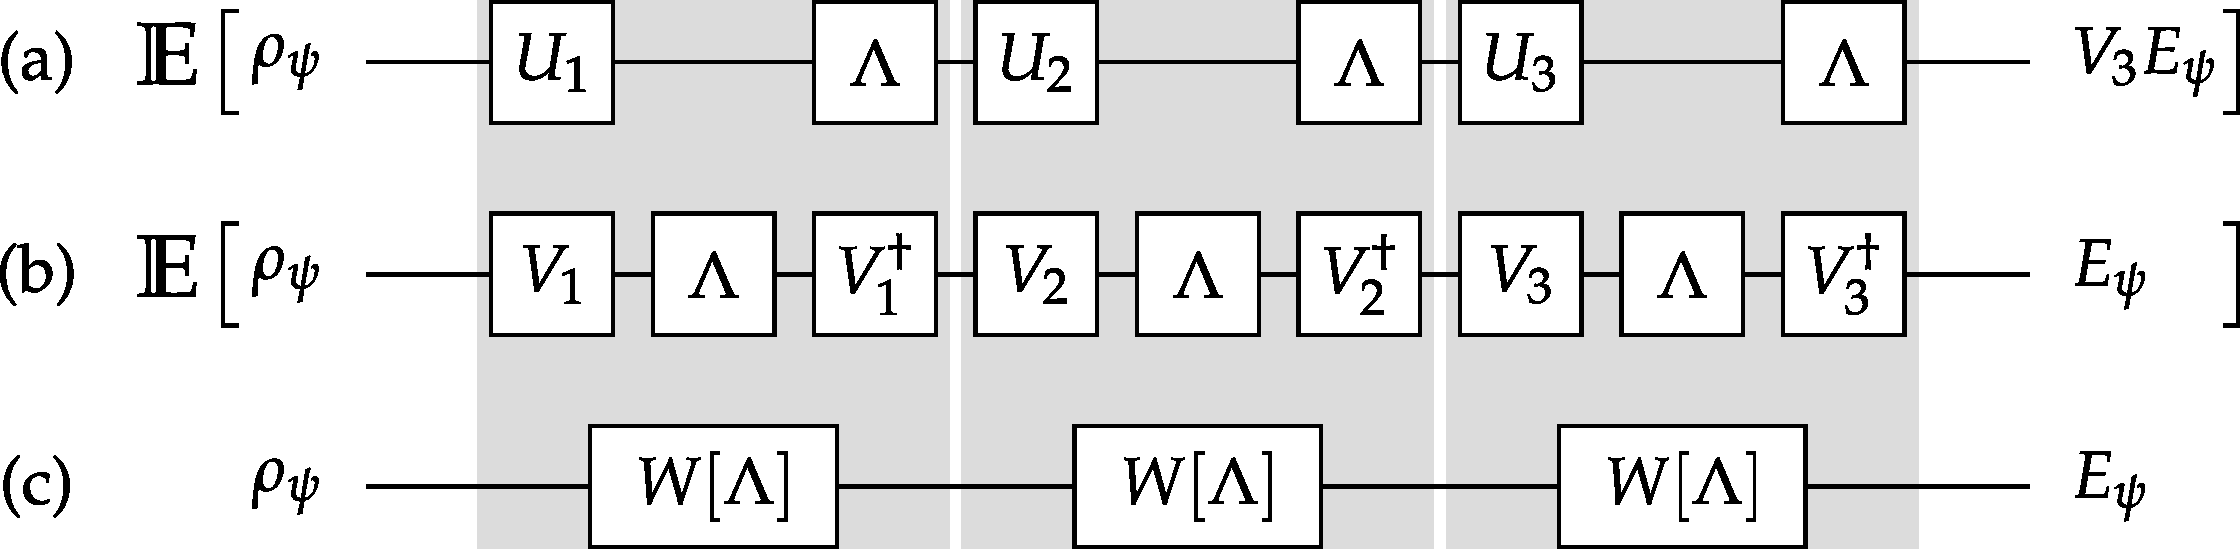
\includegraphics[width=0.85\textwidth]{figures/rb-0order-deriv}
  \end{figure}

  \bottomnote{(Knill et al. 2008 \shortdoi{cxz9vm}; Magesan et al. 2012 \shortdoi{tfz}; Magesan et al. 2012 \shortdoi{s8j})}

\end{frame}

\begin{frame}{Randomized Benchmarking Likelihood}

  Interpret survival probability as likelihood.
  For interleaved case, the lowest-order model is:
  \[
    \Pr(\text{survival} | A, B, \tilde{p}, p_{\text{ref}}; m, \text{mode}) =
    \begin{cases}
      A p_{\text{ref}}^m + B & \text{reference} \\
      A (\tilde{p} p_{\text{ref}})^m + B & \text{interleaved}
    \end{cases}
  \]

  \begin{description}
    \item[$A,B$] state preparation and measurement
    \item[$m$] sequence length
    \item[$p_{\text{ref}}$] reference depolarizing parameter
    \item[$\tilde{p}$] depolarizing parameter for gate of interest
  \end{description}

  \uncover<2->{
    $$
      \vec{x} = (A, B, \tilde{p}, p_{\text{ref}}) \quad \vec{e} = (m, \text{mode})
    $$
  }

  \bottomnote{(\emph{Granade}, Ferrie and Cory 2014 \arxiv{1404.5275})}

\end{frame}


\begin{frame}{Updating Knowledge}
 
  Once we have a likelihood, we can now reason about
  \[
    \Pr(\vec{x} | d, \vec{e}),
  \]
  what we know having seen some data.
  
  \pause\vskip0.5em

  % Formatting solution courtesy of SE user egreg:
  % http://tex.stackexchange.com/a/55503/615
  \makebox[0pt][l]{By Bayes' Rule:}%
  \makebox[\textwidth][c]{$
    \alert<4>{\Pr(\vec{x} | d, \vec{e})} = \frac{\alert<3>{\Pr(d | \vec{x}; \vec{e})}}{\Pr(d | \vec{e})} \Pr(\vec{x}).
  $}

  $\Longrightarrow$ \alert<3>{Simulation} is a resource for \alert<4>{learning}.
  
  \uncover<5->{\vskip0.5em
  
  Estimate $\hat{\vec{x}}$ as the expectation over $\vec{x}$,
  \[
      \hat{\vec{x}} = \expect[\vec{x}] = \int \vec{x} \Pr(\vec{x}) \ \dd\vec{x}.
  \]}

  \uncover<6->{
    In many cases, difficult to perform analytically...
  }


\end{frame}

\subsection{SMC Algorithm}


\begin{frame}{Sequential Monte Carlo}

  \textbf{SMC} (aka \emph{particle filter})\textbf{:} numerical algorithm for generating samples from a distribution,
  using a transition kernel.

  $$
    \text{prior} \overset{\text{Bayes' Rule}}{\longrightarrow} \text{posterior}
  $$

  \vskip0.5em

  Posterior samples then approximate $\int/\expect$.

  \begin{block}{SMC Approximation}
    $$
      \Pr(\vec{x}) \approx \sum_i^n w_i \delta(\vec{x} - \vec{x}_i)
    $$
  \end{block}

  \pause
  \begin{description}
    \item[QInfer] Open-source implementation for quantum info.
  \end{description}
  
  \bottomnote{(Doucet and Johansen 2011; Huszár and Houlsby \shortdoi{s86}; \emph{Granade} et al. 2012 \shortdoi{s87})}
\end{frame}

\begin{frame}{Ambiguity and Impovrishment}

  Ambiguity in SMC approximation:
  \begin{figure}%
    \makebox[\textwidth][c]{
      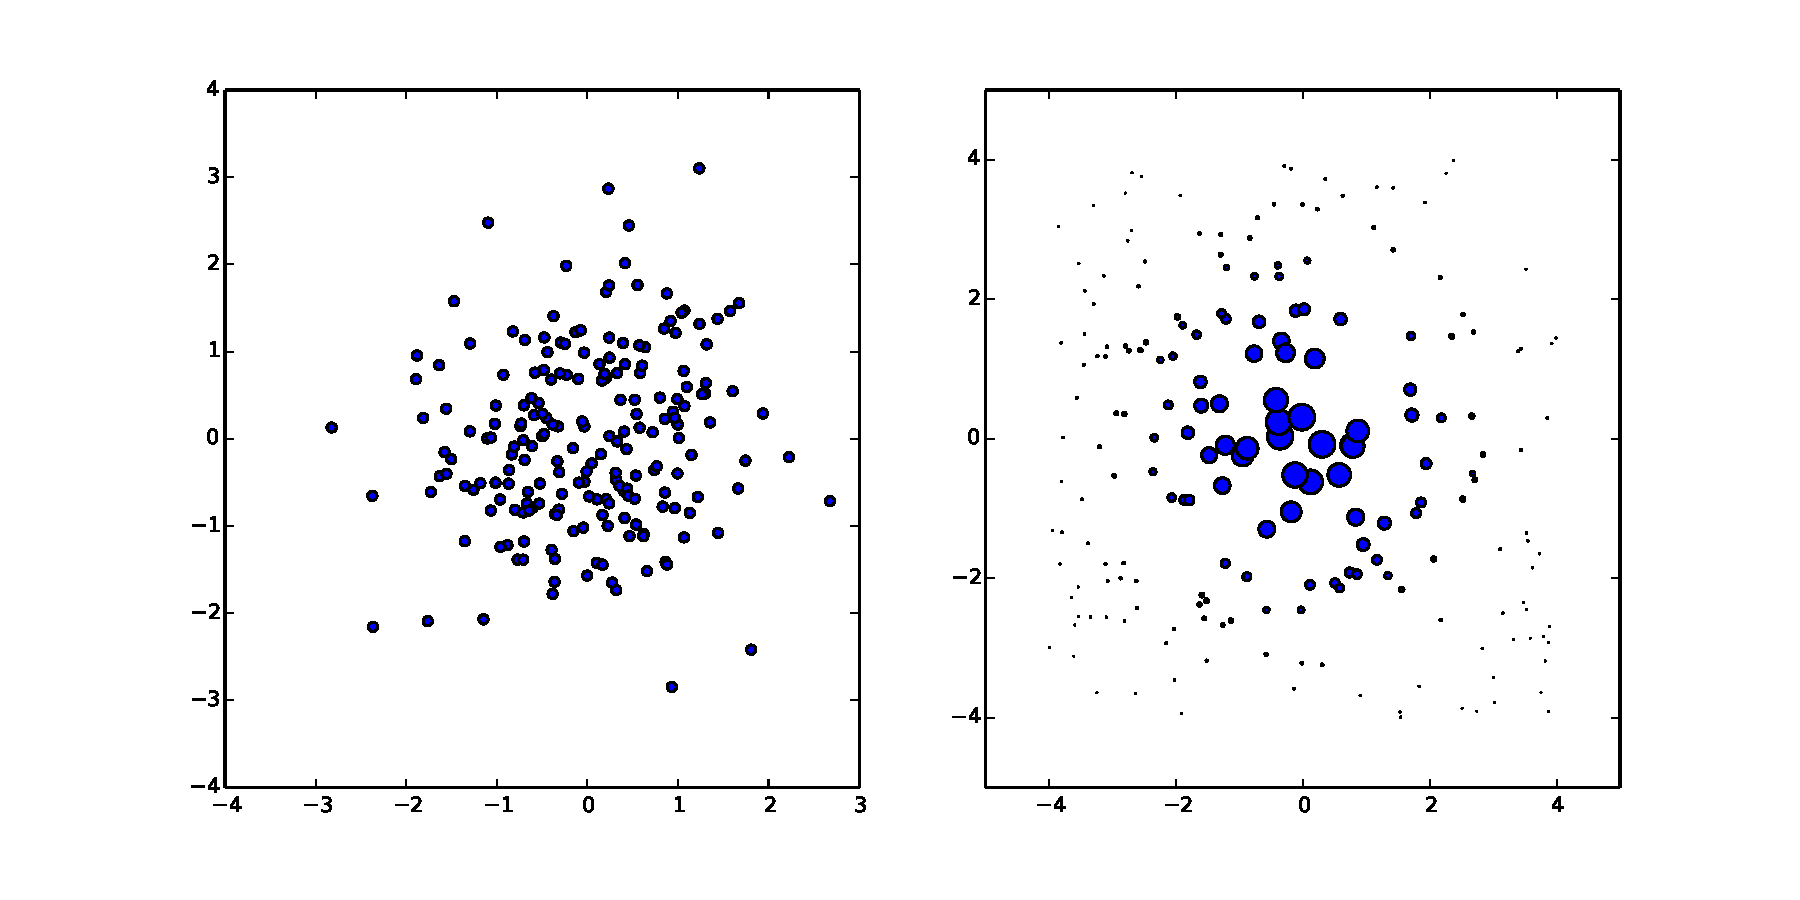
\includegraphics[width=0.7\textwidth]{figures/impovrishment}
    }

    \vspace{-0.75em}%
    \makebox[0.2\textwidth][c]{}%
    \makebox[0.3\textwidth][c]{density}%
    %\makebox[0.1\textwidth][c]{}%
    \makebox[0.3\textwidth][c]{weight}%
    \makebox[0.2\textwidth][c]{}
  \end{figure}

  \pause

  Using weight is less numerically stable, results in smaller \emph{effective}
  number of particles.

  \[
    n_{\text{ess}} \defeq 1 / \sum_i w_i^2
  \]

\end{frame}

\begin{frame}{Numerical Stability and Resampling}

  As data $D$ is collected, $\Pr(\vec{x}_i | D) \to 0$ for most
  initial particles $\{x_i\}$.

  \begin{itemize}
    \item $\Rightarrow n_{\text{ess}} \to 0$ as data is collected.
  \end{itemize}

  \emph{Resampling}: move information from weights
  to the density of SMC particles.

  \begin{itemize}
    \item Resampling when $n_{\text{ess}} / n \le 0.5$ preserves stability.
    \item Monitoring $n_{\text{ess}}$ can herald some kinds of failures.
  \end{itemize}

\end{frame}
 
\begin{frame}{Liu and West Algorithm}
  
  Draw new particles $\vec{x}'$ from kernel density estimate:
  \begin{gather*}
    \Pr(\vec{x}') \propto \sum_i w_i \exp\left((\vec{x}' - \vec{\mu}_i)^\T\matr{\Sigma}(\vec{x}' - \vec{\mu}_i)\right) \\
    \vec{\mu}_i \defeq a \vec{x}_i + (1 - a) \mathbb{E}[\vec{x}] \qquad
    \matr{\Sigma} \defeq h^2 \Cov[\vec{x}] \qquad
    w_i' \defeq 1 / n
  \end{gather*}

  \pause

  Parameters $a$ and $h$ can be set based on application:
  \begin{itemize}
    \item $a = 1, h = 0$: Bootstrap filter, used in state-space applications
      like \textsc{Condensation}.
    \item $a^2 + h^2 = 1$: Ensures $\expect[\vec{x}'] = \expect[\vec{x}]$
      and $\Cov(\vec{x}') = \Cov(\vec{x})$, but assumes unimodality.
    \item $a = 1, h \ge 0$: Allows for multimodality, emulating state-space
      with synthesized noise.
  \end{itemize}
  
  \bottomnote{(West 1993;  Isard and Blake 1998 \shortdoi{cc76f6}; Liu and West 2001)}
  
\end{frame}

\begin{frame}{Putting it All Together: The SMC Algorithm}

  \begin{enumerate}
    \item Draw $\{\vec{x}_i\} \sim \pi$, set $\{w_i\} = 1/n$.
    \item For each datum $d_j \in D$:
    \begin{enumerate}
      \item $w_i \gets w_i \times \Pr(d_j | \vec{x}_i; \vec{e}_j)$.
      \item Renormalize $\{w_i\}$.
      \item If $n_{\text{ess}} / n \le 0.5$, resample.
    \end{enumerate}
    \item Report $\hat{\vec{x}} \defeq \expect[\vec{x}] \approx \sum_i w_i \vec{x}_i$.
  \end{enumerate}

\end{frame}

\subsection{Examples}

\begin{frame}{Sequential Monte Carlo}
  
  With SMC and resampling, particles move towards the true model as data is collected.
  
  \begin{figure}
    \includegraphics<1>[width=0.6\textwidth]{figures/1D_SMC_1_v2}
    \includegraphics<2>[width=0.6\textwidth]{figures/1D_SMC_6_v2}
    \includegraphics<3>[width=0.6\textwidth]{figures/1D_SMC_11_v2}
  \end{figure}
  
\end{frame}

\begin{frame}{}

  Before bootstrapping, a few examples of SMC w/ classical resources:

\end{frame}

\begin{frame}{Randomized Benchmarking Results}

  Using SMC, useful conclusions can be reached with significantly
  less data than with least-squares fitting.

  \begin{figure}
    \centering
    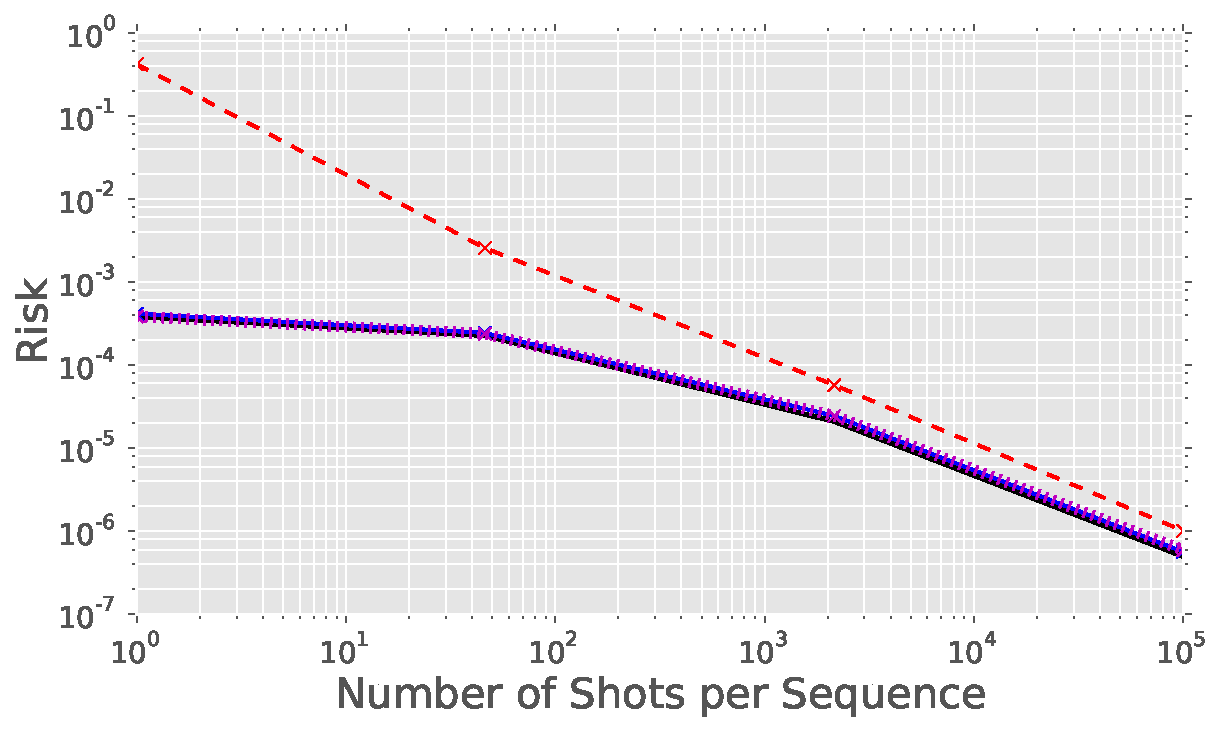
\includegraphics[width=0.8\textwidth]{figures/risk-tr-comparison} \\
    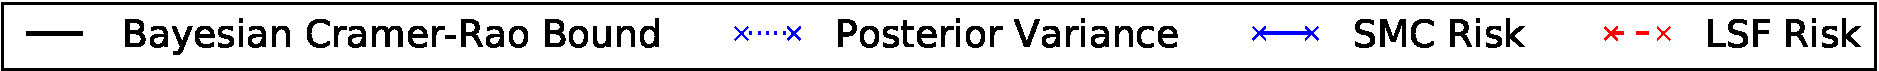
\includegraphics[width=0.8\textwidth]{figures/risk-comparison-legend-crop}
  \end{figure}

  \bottomnote{(\emph{Granade}, Ferrie and Cory 2014 \arxiv{1404.5275})}

\end{frame}

\begin{frame}{Randomized Benchmarking Results}

    SMC is robust, even with a quite bad prior ($6.9\sigma$).

    \begin{figure}
        \centering
        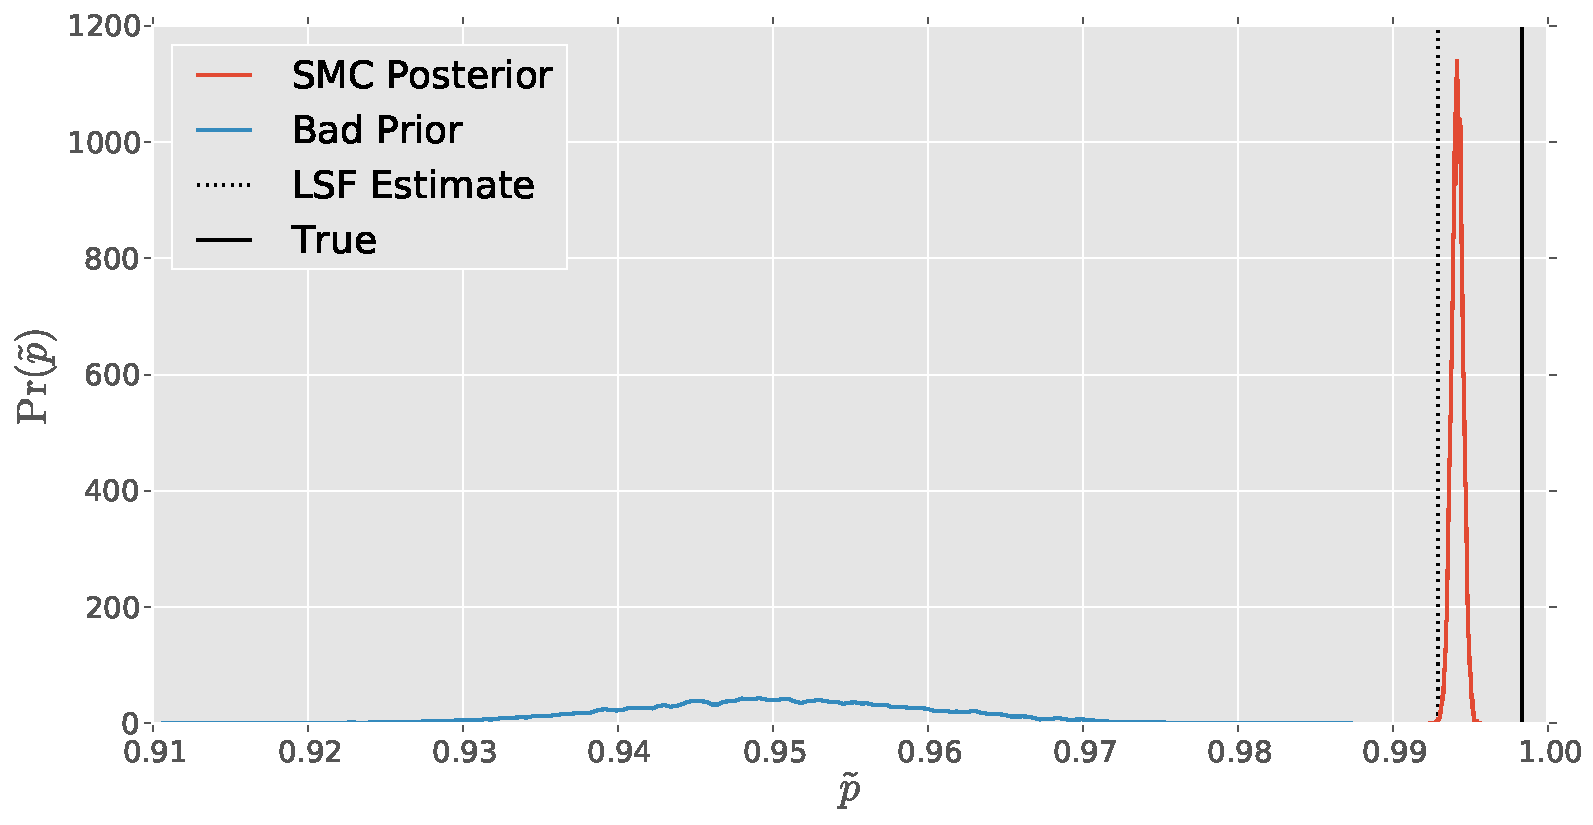
\includegraphics[width=0.8\textwidth]{figures/bad-prior-distns}
    \end{figure}

    \pause
    \begin{itemize}
        \item Monitoring $n_{\text{ess}}$ can herald failures due to a bad prior.
    \end{itemize}

\end{frame}

\begin{frame}{SMC in Nitrogen Vacancy Centers}

  Would like to learn hyperfine coupling $\matr{A}$
  between $e^{-}$ spin $\vec{S}$ and ${}^{13}\text{C}$ spin $\vec{I}$.

  \begin{align*}
    H(\vec{x}) & = \Delta_{\text{zfs}} S_z^2 + \gamma (\vec{B} + \vec{\delta B}) \cdot \vec{S} + \vec{S} \cdot \matr{A} \cdot \vec{I} \\
    \vec{x} & = (\Delta_{\text{zfs}}, \vec{\delta B}, \matr{A}, \alpha, \beta, T_{2,e}^{-1}, T_{2,C}^{-1}) \\
    \alpha,\beta & : \text{visibility parameters}
  \end{align*}

  \pause

  \begin{itemize}
    \item Analytic estimate sensitive to error $\vec{\delta B}$ in static field.
    \item Use multiple $\vec{B}$ settings to decorrelate $\vec{\delta B}$, $\matr{A}$.
    \item Each experiment informs about multiple parameters.
  \end{itemize}

\end{frame}

\begin{frame}{Preliminary Results from Rabi Experiment}

  \only<1>{
    As a test, attempt to learn $\vec{\delta B}$, $\Delta_{\text{zfs}}$
    $\delta\omega_{\text{Rabi}}$ and $A_N$ (coupling to nitrogen spin).
  }

  \only<2->{
    \begin{figure}
      \centering
      %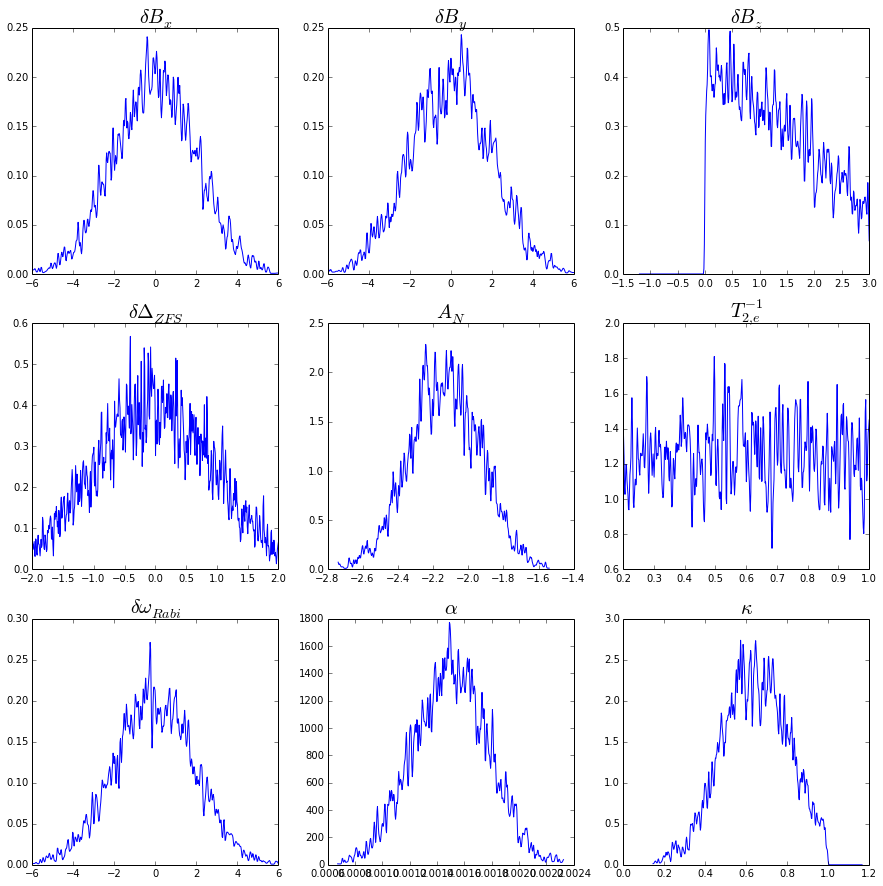
\includegraphics[height=2.5cm]{figures/marginals5000_000}
      \includegraphics<2>[height=3.5cm]{figures/simulation_fourier5000_000}
      \includegraphics<3>[height=3.5cm]{figures/simulation_fourier5000_020}
      \includegraphics<4>[height=3.5cm]{figures/simulation_fourier5000_486}
      \includegraphics<5>[height=6cm]{figures/marginals5000_000}
      \includegraphics<6>[height=6cm]{figures/marginals5000_020}
      \includegraphics<7>[height=6cm]{figures/marginals5000_486}

      \only<2>{Simulation with prior mean}
      \only<3>{Simulation with posterior mean, 20 averages}
      \only<4>{Simulation with posterior mean, 486 averages}
      \only<5>{Marginals of prior}
      \only<6>{Marginals of posterior, 20 averages}
      \only<7>{Marginals of posterior, 486 averages}
    \end{figure}

    \bottomnote{Each average: 30k shots per point, 100 Rabi points + 200 Ramsey points}
  }

\end{frame}

\begin{frame}{SMC and Hamiltonian Learning as Vector Metrology}

  In the previous example, $\delta B_x$ and $\delta B_y$ manifest
  as effective Hamiltonian by Floquet theory.

  \pause

  \begin{block}{}
    Each experiment carries phase information about $\vec{\delta B}$.

    \vskip0.5em

    SMC uses this to learn vector quantities: we do not require
    that each component of $\vec{\delta B}$ be measured seperately.
  \end{block}

\end{frame}

\subsection{}

\begin{frame}{Towards Bootstrapping}
  
  SMC uses \emph{simulation} as a resource for \emph{learning}.

  \vskip0.5em

  Simulation calls: main cost to SMC ($n$ each Bayes update).

  \vskip0.5em\pause
  
  \begin{block}{Big Idea}
    Use quantum simulation to extend SMC past classical resources.
  \end{block}
  
\end{frame}

\section[QHL]{Quantum Hamiltonian Learning}

\subsection[Weak Sim.]{Weak and Strong Simulation}

\begin{frame}{Weak and Strong \only<3->{Analog[ue]? }Simulation}

  \begin{figure}
    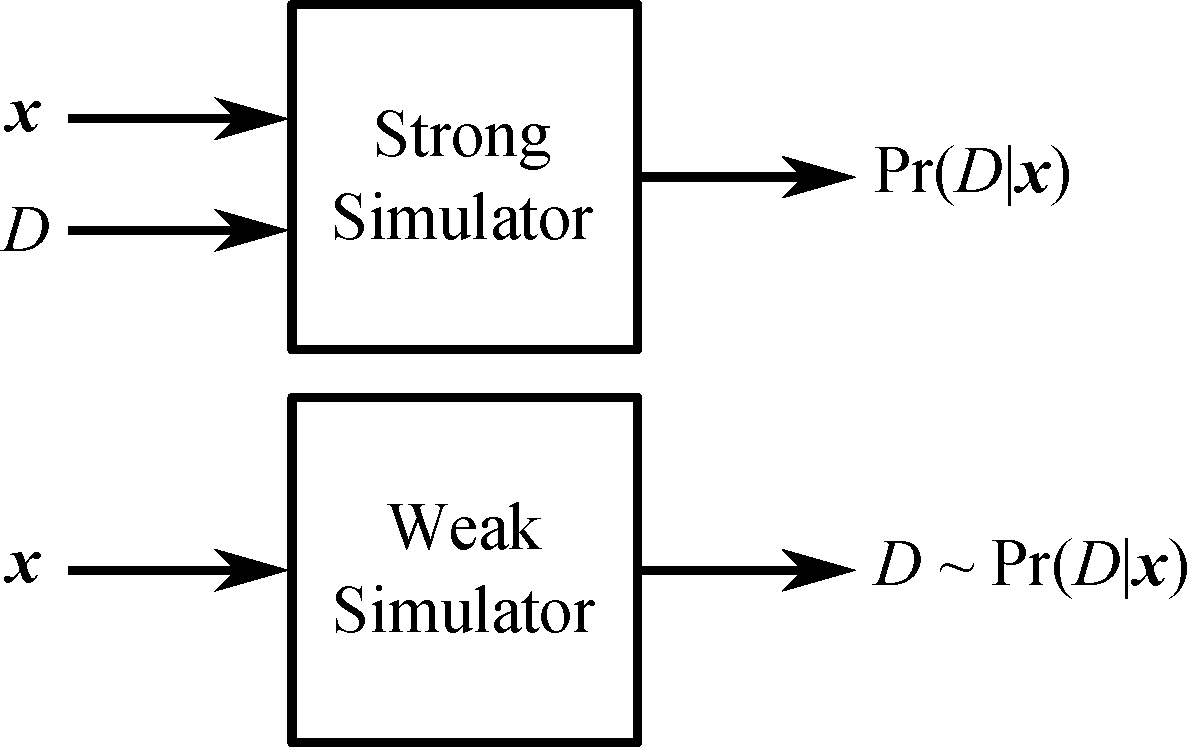
\includegraphics[width=2in]{figures/simulators}
  \end{figure}

  \vskip0.5em
  
  \uncover<2->{
    Quantum simulation produces data, not likelihoods.
    Must sample to estimate likelihood.
  }

  \vskip0.5em
  \uncover<3->{
    Potential application for analog[ue] simulators?
  }
  
  \bottomnote{(Ferrie and \emph{Granade} 2014 \shortdoi{tdj})}

\end{frame}

\begin{frame}{Adaptive Likelihood Estimation}

  \begin{block}{Solution}
    Treat estimating the likelihood as a secondary estimation
    problem:

    \vskip0.25em

    Learn likelihood of untrusted system from frequencies of trusted system.
  \end{block}

  \pause

  SMC is robust to likelihood estimation errors.

\end{frame}

\begin{frame}{Performance of SMC+ALE}

  \textbf{Ex:} Simple `photodetector' model
  $
      \Pr(0 | p) = \alpha p + (1-p) \beta
  $
  \begin{figure}
    \centering
    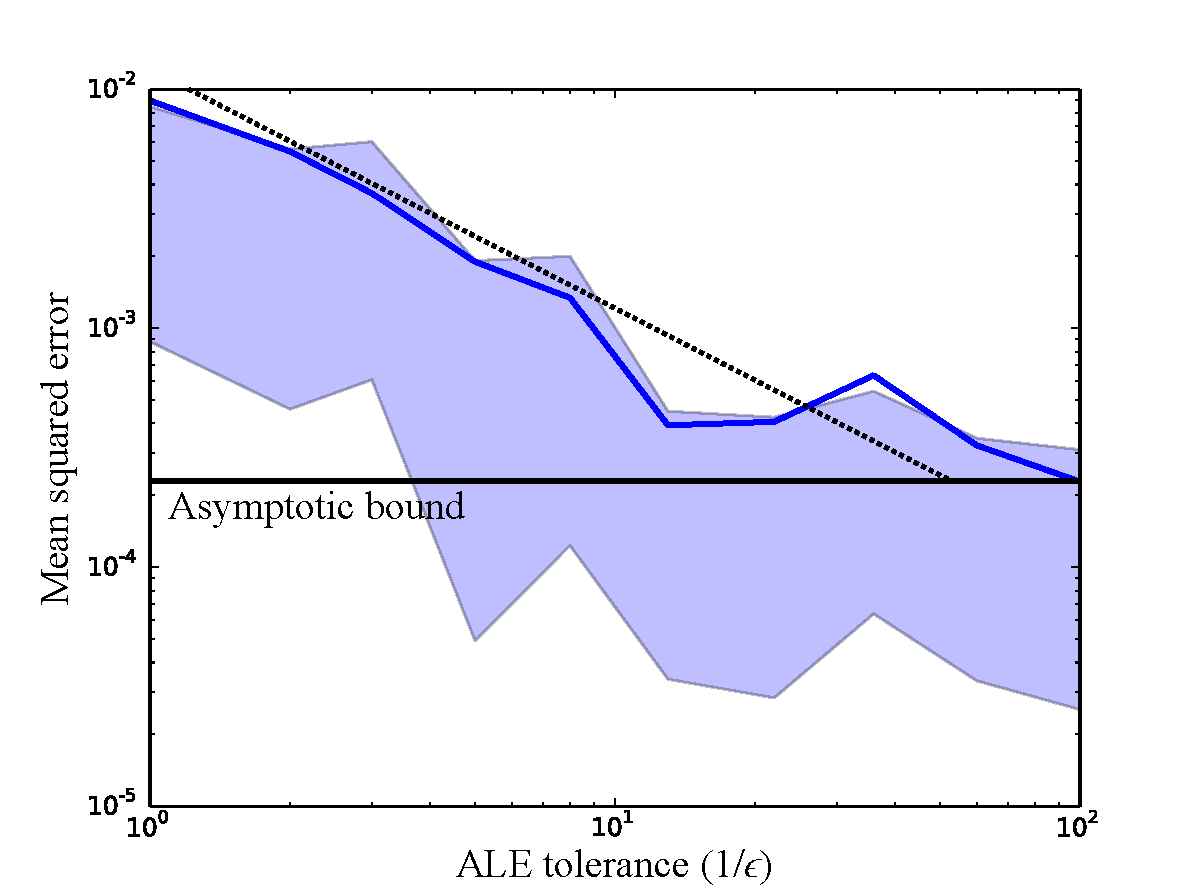
\includegraphics[width=0.6\textwidth]{figures/nc_risk_v_ale_eps}
  \end{figure}
  \begin{description}
      \item[$\alpha,\beta$] known bright, dark references
  \end{description}

  \bottomnote{(Ferrie and Granade 2014 \shortdoi{tdj})}
    
\end{frame}

\begin{frame}{ALE Example: Two-Outcome Models}
  
  Given:
  \begin{description}
    \item[$d$] result of measurement
    \item[$D'$] set of samples from weak simulator
  \end{description}

  Hedged binomial estimate of likelihood $\ell$
  from frequency $k / K$:
  \[
    \hat{\ell} = \frac{k + \beta}{K + 2 \beta},
  \]
  where $\beta \approx 0.509$, $k \defeq |\{d' \in D' | d' = d\}|$, $K = |\{D'\}|$.
  
  \pause \vskip0.5em
  
  Variance well-known, so collect until a fixed \emph{tolerance} is reached.
  
  \bottomnote{(Ferrie and Blume-Kohout 2012 \shortdoi{tf2}, Ferrie and Granade 2014 \shortdoi{tdj})}
\end{frame}

\subsection[Likelihood]{Likelihood Evaluation}

\begin{frame}{Quantum Likelihood Evaluation}
  
    Compare \emph{classical} outcomes of unknown and trusted
    systems.
  \[
      \begin{matrix}
  \text{Unknown System} &
  &
  \text{Simulator} \\
  \vphantom{\rule{0pt}{2.5em}}\Qcircuit @R 1em @C 1.5em {
        & \ustick{t}                                     &        &     \\
      \lstick{\ket{\psi}} & \gate{e^{-i H(\vec{x}_0) t}} \cwx[-1] & \meter & \rstick{d} \cw
  } &
  \qquad &
  \Qcircuit @R 1em @C 1.5em {
        & \ustick{t, \vec{x}_i}                                     &        &     \\
      \lstick{\ket{\psi}} & \gate{e^{-i H(\vec{x}_i) t}} \cwx[-1] & \meter & \rstick{D'_i} \cw
  } 
      \end{matrix}
    \]

    \vskip0.5em

    For each $\vec{x}_i$:
    \begin{itemize}
      \item repeatedly sample from quantum simulation
      of $\ee^{-\ii t \vec{x}_i}$, getting $D'_i$.
      \item estimate $\hat{\ell_i}$ from $D'_i$.
    \end{itemize}



    \makebox[0pt][l]{SMC update:}%
    \makebox[\textwidth][c]{$
      w_i \mapsto w_i \hat{\ell}_i / \sum_i w_i \hat{\ell}_i.
    $}

  \bottomnote{(Wiebe, \emph{Granade}, Ferrie and Cory 2014 \shortdoi{tf3})}
  
    
\end{frame}

\begin{frame}

  QLE can work, but as $t\to\infty$, $\Pr(d | \vec{x}; t) \rightsquigarrow 1 / \dim{\Hil}$.\\
  Thus, $t \ge t_{\text{eq}}$ is uninformative.

  \vskip0.5em

  By CRB, error then scales as $\OO(1 / N t_{\text{eq}}^2)$.

\end{frame}

\begin{frame}{Interactive QLE}

    Solution: couple unknown system to a
    quantum simulator, then invert evolution by hypothesis $\vec{x}_-$.
    
    \[
      \Qcircuit @R 1em @C 1.5em {
                        &                                      &                & \ustick{t, \vec{x}_-}                 &        &                &  \\
                        & \qw                                  & \qswap \qwx[1] & \gate{e^{+i H(\vec{x}_-) t}} \cwx[-1] & \meter & \rstick{d} \cw &  \\
    \lstick{\ket{\psi}} & \gate{e^{-i H(\vec{x}_0) t}} \cwx[1] & \qswap         & \qw                                   & \qw    & \qw            &  \\
                        & \dstick{t}                           &                &                                       &        &                &
      }
    \]
    \vskip1em\pause

    \begin{block}{Echo}
    If $\vec{x}_- \approx \vec{x}_0$, then
    $\left|\braket{\psi | \ee^{-\ii t (H(\vec{x}_0) - H(\vec{x}_-))} | \psi}\right|^2 \approx 1$.
    \end{block}

  \bottomnote{(Wiebe, \emph{Granade}, Ferrie and Cory 2014 \shortdoi{tf3})}

\end{frame}

\begin{frame}{Posterior Guess Heuristic}
 
    Inversion connects the model and experiment spaces.

    Use this duality as a heuristic for experiment design.
    
    \begin{itemize}
     \item Choose $\vec{x}_-, \vec{x}_-' \sim \Pr(\vec{x})$, the most recent posterior.
     \item Choose $t = 1 / \|\vec{x}_- - \vec{x}_-'\|$.
     \item Return $\vec{e} = (\vec{x}_-, t)$.
    \end{itemize}

  \bottomnote{(Wiebe, \emph{Granade}, Ferrie and Cory 2014 \shortdoi{tf3})}

 
\end{frame}

\begin{frame}{Alternate Interpretation}

    QHL finds $\hat{\vec{x}}$ such that $H(\hat{\vec{x}})$ most closely
    approximates ``unknown'' system $H_0$.

    \vskip0.5em

    Gives an $\alpha$-credible bound on error introduced by replacing $H_0 \to H(\hat{\vec{x}})$.

\end{frame}

\subsection{Results}

\begin{frame}{Ising Model on Spin Chains}

    Hamiltonian: nearest-neighbor Ising models on a chain
    of nine qubits.

    Interactivity allows for dramatic improvements over
    QLE.
    
    \begin{figure}
      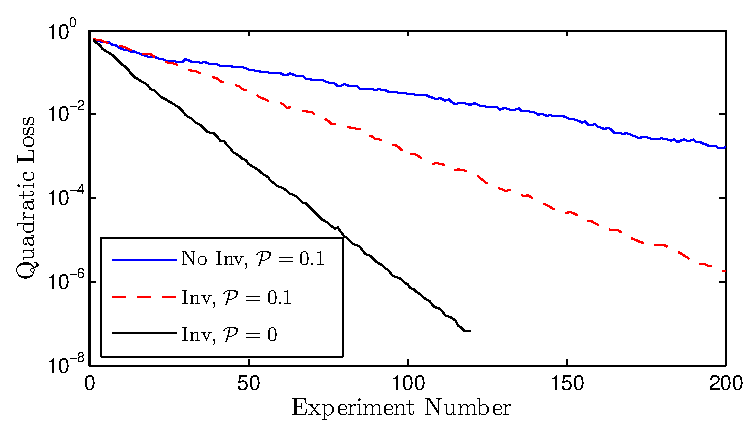
\includegraphics[width=0.725\textwidth]{figures/poison}
    \end{figure}

    $\mathcal{P}$: adaptive likelihood estimation tolerance.

  \bottomnote{(Wiebe, \emph{Granade}, Ferrie and Cory 2014 \shortdoi{tf3})}

\end{frame}

\begin{frame}{Ising Model on the Complete Graph}
    
    With IQLE, can also learn on complete interaction graphs.
    We show the performance as a function of
    the depolarization strength $\mathcal{N}$.
    
    \begin{figure}
      \centering
      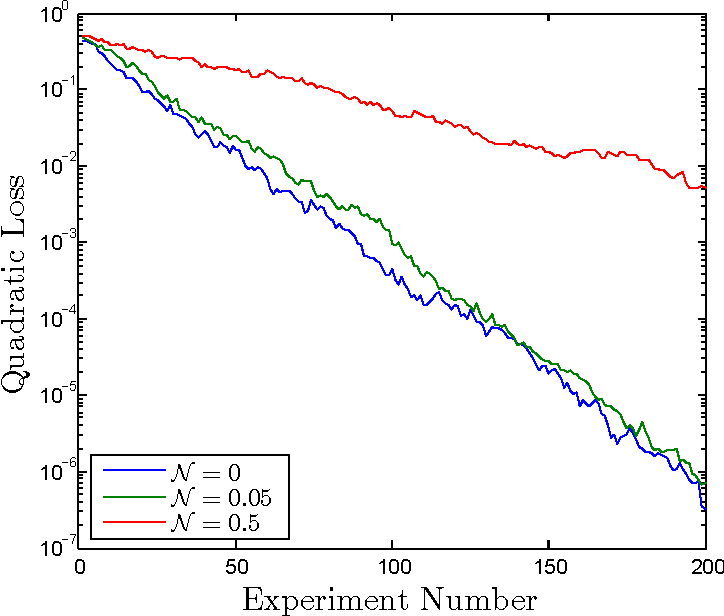
\includegraphics[width=0.45\textwidth]{figures/tpnoise}
    \end{figure}

    $\mathcal{N}$: depolarizing noise following SWAP gate.

  \bottomnote{(Wiebe, \emph{Granade}, Ferrie and Cory 2014 \shortdoi{tdk})}
    
\end{frame}

\begin{frame}{Ising Model with the Wrong Graph}

  Simulate with spin chains, suppose ``true'' system is complete,
  with non-NN couplings $\OO(10^{-4})$.

  \begin{figure}
    \centering
    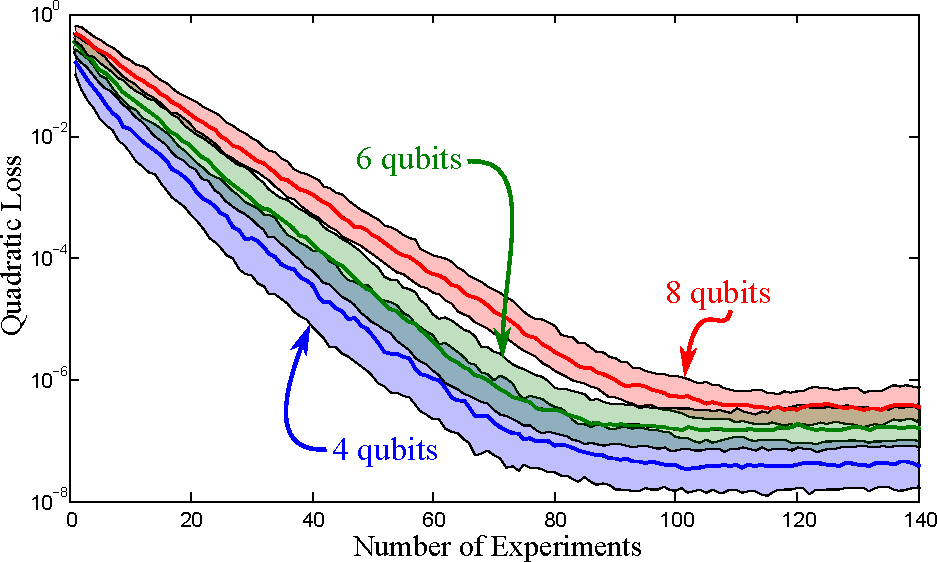
\includegraphics[width=0.7\textwidth]{figures/badmodel}
  \end{figure}

  \bottomnote{(Wiebe, \emph{Granade}, Ferrie and Cory 2014 \shortdoi{tdk})}

\end{frame}

\begin{frame}{Scaling Parameter}

  \begin{block}{}
     $\dim \vec{x}$, not $\dim \Hil$, determines scaling of IQLE.
  \end{block}

  \begin{figure}
    \centering
    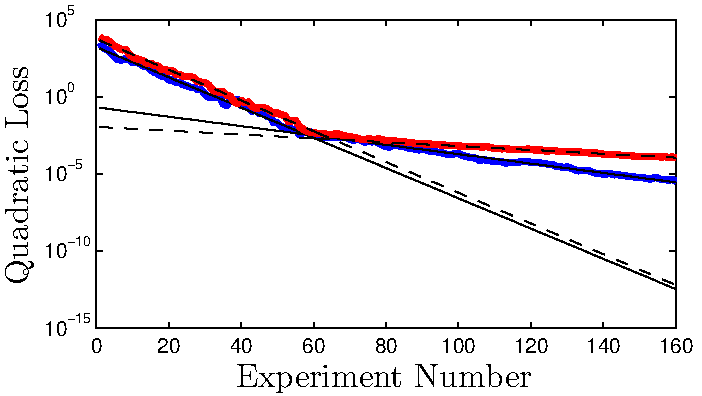
\includegraphics[width=0.6\textwidth]{figures/corner}
    \caption{4 qubit (red) and 6 qubit (blue) complete graph IQLE}
  \end{figure}

  \bottomnote{(Wiebe, \emph{Granade}, Ferrie and Cory 2014 \shortdoi{tf3})}

\end{frame}

\begin{frame}{Scaling and Dimensionality}

    In spin-chain and complete graph, average error decays exponentially,
    \[
      L(N) \propto e^{-\gamma N}
    \]
    \pause
    Assess scaling by finding $\gamma = \gamma(\dim\vec{x})$:
    \begin{figure}
      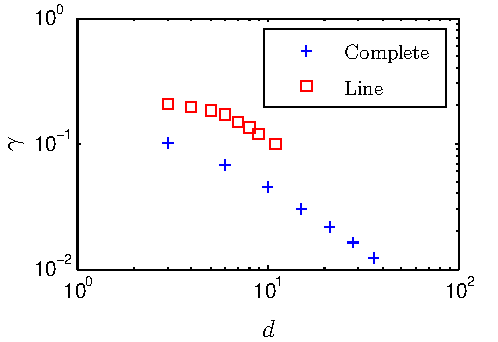
\includegraphics[width=0.55\textwidth]{figures/exp_scale}
    \end{figure}
    \vspace{-1.5em}
    With quantum simulation, learning \emph{may} scale efficiently.

  \bottomnote{(Wiebe, \emph{Granade}, Ferrie and Cory 2014 \shortdoi{tf3})}

\end{frame}

\begin{frame}

  SMC + IQLE:

  \begin{itemize}
    \item Possibly scalable with quantum resources.
    \item Robust to finite sampling.
    \item Robust to approximate models.
  \end{itemize}

  \begin{block}{}
    Still requires simulator be at least as large as system of interest.
  \end{block}

\end{frame}

\section{Bootstrapping}

\subsection{Overview}

\begin{frame}{Information Locality}
  
  To go further, we want to \emph{localize} our experiment,
  such that we can simulate on a smaller system.

  \begin{figure}
    \centering
    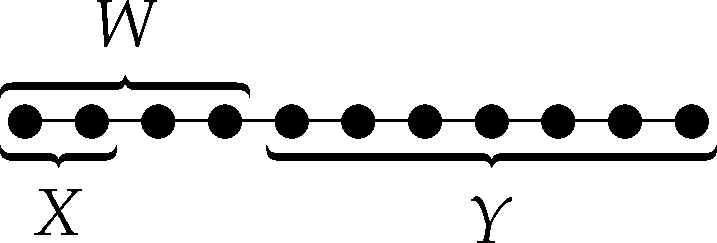
\includegraphics[width=0.6\textwidth]{figures/bootstrapping-partition}
  \end{figure}

  Measure on $X$, simulate on $W$, and ignore all terms with support
  over $Y$.

  \vskip0.5em
  \pause

  Gives \emph{approximate} model that can be used to learn Hamiltonian
  restricted to $X$.

\end{frame}

\begin{frame}{Local and Global Particle Clouds}
  
  To reconstruct the entire system, we need to combine data from different partitions.
  
  \begin{figure}
    \centering
    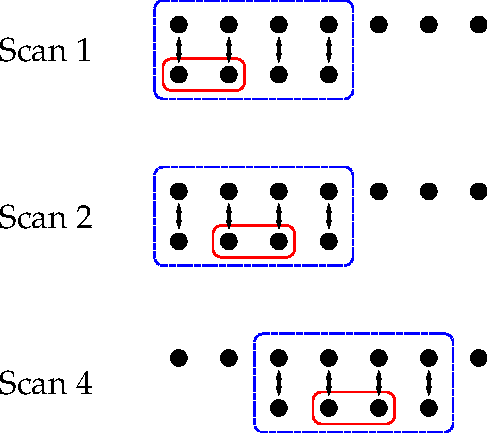
\includegraphics[width=0.4\textwidth]{figures/scanning}
  \end{figure}

  Separate out one partition at a time, maintain a \emph{global} cloud of particles. 
  
\end{frame}

\begin{frame}{Local and Global Particle Clouds}

  Initialize $\{\vec{x}_i\}$ over entire system. Then, for each simulated subregister $W_k$:
  \begin{enumerate}
    \item Make ``local'' particle cloud $\{\vec{x}_i|_{W_k}\}$ by slicing $\{\vec{x}_i\}$.
    \item Run SMC+IQLE with $\{\vec{x}_i|_{W_k}\}$ as a prior.
    \item Ensure that the final ``local'' cloud has been resampled (has equal weights).
    \item Overwrite parameters in ``global'' cloud $\{\vec{x}_i\}$ corresponding
      to post-resampling $\{\vec{x}_i|_{W_k}\}$.
  \end{enumerate}

  In this way, all parameters are updated by an SMC run.

\end{frame}

\subsection{Example}

\begin{frame}{Q50 Example}

  Goal: characterize a 50-qubit Ising model (complete graph) with unknown $ZZ$ couplings.

  \vskip0.5em

  All Hamiltonian terms commute, but initial state doesn't.
  Let $A_X$ be observable, $A_{X'}$ be sim. observable.

  \begin{align*}
    \|A_X(t) - A_{X'}(t)\| & \le \|A_X(t)\| (\ee^{2\|H|_{Y}\|t} - 1) \\
    \Rightarrow t & \le \ln\left(\frac{\delta}{\|A_X(t)\|} + 1\right) (2\|H|_{Y}\|)^{-1},
  \end{align*}

  where $\delta$ is the tolerable likelihood error.

\end{frame}

\begin{frame}{Example Q50 Run}

  \begin{figure}
    \centering
    \includegraphics<1>[width=1\textwidth]{figures/8outc2a-hist}
    \includegraphics<2>[width=0.5\textwidth]{figures/q50-comparison}
  \end{figure}

  $|X_k| = 4$, $|W_k| = 8$, $n = 20,000$, $N = 500$, exp. decaying interactions.\\
  NB: 1225 parameter model, $L_2$ error of $0.3\%$.

\end{frame}

\begin{frame}{Scaling With $N$}

    We expect from non-truncated quantum Hamiltonian learning that the error
    decays exponentially with more data. This remains the case even with truncation.

    \begin{figure}
        \centering
        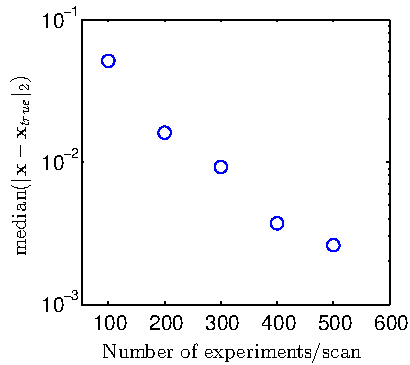
\includegraphics[width=0.6\textwidth]{figures/errperexp}
    \end{figure}

\end{frame}

\subsection{Non-Commuting $H$}

\begin{frame}{Lieb-Robinson Bounds}

  More generally, for $[H|_W, H_Y] \ne 0$, use \emph{Lieb-Robinson bound}.

  If interactions between $X$ and $Y$ decay sufficiently quickly,
  then there exists $C$, $\mu$ and $v$ s. t. for any observables $A_X(t)$, $B_Y$:
  $$
    \|[A_X(t), B_Y]\| \le C \|A_X(t)\| \|B_Y\| |X| |Y| (\ee^{v|t|} - 1) \ee^{-\mu d(X, Y)}
  $$

  This \emph{guarantees} that error due to truncation is bounded if
  we choose small $t$.

  \bottomnote{(Hastings and Koma 2006 \shortdoi{cddqgz}; Nachtergale and Sims 2006 \shortdoi{d9xwfg})}

\end{frame}

\begin{frame}{Lieb-Robinson Bounds}

  Can find bound in terms of Hamiltonian by considering $H$ site-by-site.

  \begin{figure}
    \centering
    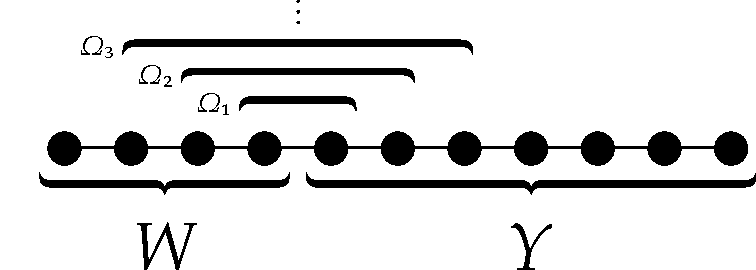
\includegraphics[width=0.6\textwidth]{figures/bootstrapping-partition-distance}
  \end{figure}

  Let $H_j$ be the Hamiltonian term containing distance-$j$
  interactions between $W$ and $Y$, acting on sites $\Omega_j$.

  $$
    \|A(t) - \ee^{\ii H|_W t} A \ee^{-\ii H|_W t} \| \le
    \sum_{j} C \|A\| \|H_j\| |X| |\Omega_j| \ee^{-\mu j} (\ee^{v |t|} - 1)
  $$

\end{frame}

\begin{frame}

  \begin{figure}
    \centering
    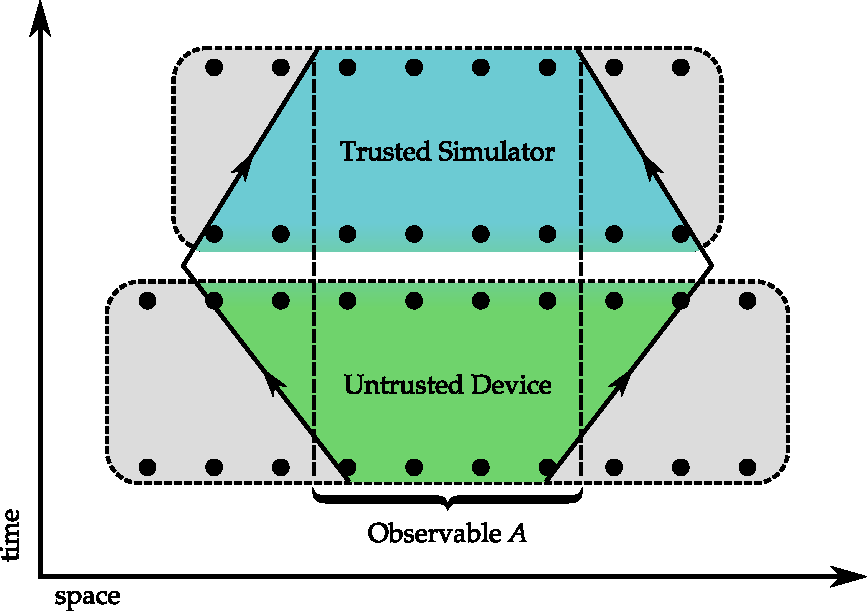
\includegraphics[width=0.8\textwidth]{figures/lightcones-vertical-v1}
  \end{figure}

\end{frame}

\begin{frame}{``Shaking''}

  Can improve the Lieb-Robinson bound by alternating between simulator
  and system. Using $r \approx vt$ $\swapgt$ gates, error is $\OO(t)$.

  \begin{figure}
    \centering
    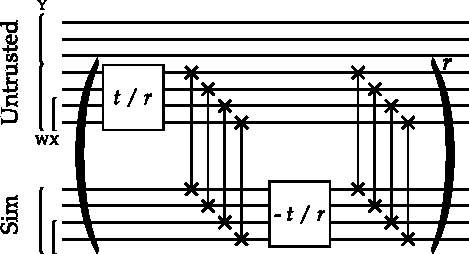
\includegraphics[width=0.8\textwidth]{figures/shaking}
  \end{figure}

\end{frame}

\subsection[Control]{Learning Controls}

\begin{frame}{Bootstrapping Algorithm}

  Consider $H$ an affine map $H(\vec{C})$ of control settings $\vec{C}$:
  \begin{equation}
      H(\vec{C}) = \vec{C} \cdot (H_1, H_2, \dots, H_M) + H_0.
  \end{equation}
  E.g.: cross-talk.

  We can learn this with truncated IQLE:
  \begin{itemize}
      \item Learn $H(\vec{0})$ to estimate $\hat{H}_0$.
      \item Learn $H(\vec{e}_j)$ for $j \in \{1, \dots, M\}$.
      \item Subtract $\hat{H}_0$ from each of the learned Hamiltonians
          to estimate the other terms.
      \item Use the pseudoinverse to derive control settings to generate
          desired Hamiltonians.
  \end{itemize}
\end{frame}

\begin{frame}{Example: Controlling NN Ising Couplings}
  
  Consider $H(\vec{C})$ such that $C_i$ nominally controls
  the coupling $H_i = \sigma_z^{(i)} \sigma_z^{(i + 1)}$. For a
  50-qubit device, $\dim\vec{C} = 49$, so this is a
  $(49 + 1) \times 1225 \approx 61 \times 10^3$ parameter model.

  \vspace{2em}

  We collect 200 bits of data per scan, for a total of
  $50 \times 49 \times 200 = 490 \times 10^3$ bits of data.
  We use $20\times 10^3$ particles, for a total of
  10 million likelihood calls.

\end{frame}

\begin{frame}{Results for Bootstrapping 50-Qubit Simulator}

  \begin{figure}
      \centering
      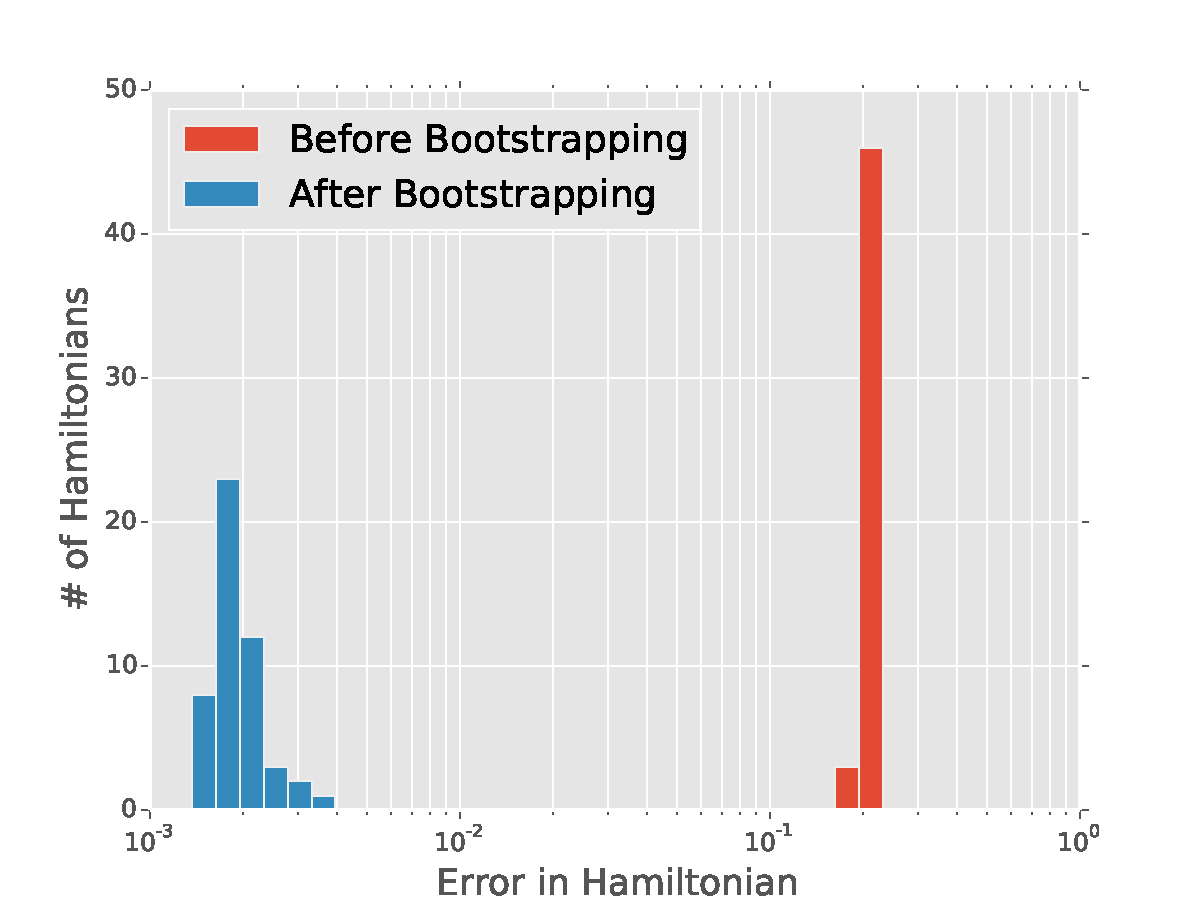
\includegraphics[width=0.8\textwidth]{figures/histplots_200}
      \caption{
        Frequencies of error $\|H(\hat{\vec{C}}_i) - H_i\|_2$ for Q50 bootstrapping.
      }
  \end{figure}

\end{frame}

\section{Conclusions}

\begin{frame}{}

  \begin{itemize}
   \item<+-> Bayesian inference: simulation as a characterization/validation resource.
   \item<+-> Sequential Monte Carlo: numerical algorithm for inference.
   \item<+-> Robust to many practical concerns.
   \item<+-> Can use quantum simulation to offer potential scaling.
   \item<+-> Using robustness of SMC, can truncate simulation $\to$ bootstrapping.
  \end{itemize}

\end{frame}

\begin{frame}{Further Information}

  Slides, a journal reference for this work, a full bibliography and a software implementation can
  be found at \url{http://www.cgranade.com/research/talks/usydney-2014/}.

  \begin{figure}
     
\includegraphics[width=0.4\textwidth]{figures/link}
  \end{figure}

  \begin{block}{}
    Thank you for your kind attention!
  \end{block}
\end{frame}


\appendix 



\begin{frame}{Decision Theory}

  A few definitions help us evaluate estimates $\hat{\vec{x}}$ of $\vec{x}$:

  \begin{description}[<+->]
    \item[Loss]       How well have we learned?
      $L_{\matr{Q}}(\hat{\vec{x}}, \vec{x}) \defeq (\hat{\vec{x}} - \vec{x})^{\T} \matr{Q} (\hat{\vec{x}} - \vec{x})$
    \item[Risk]       On average, how well will we learn a particular model?\\
      $R(\hat{\vec{x}}, \vec{x}) \defeq \expect_D [L(\hat{\vec{x}}(D), \vec{x})]$
    \item[Bayes risk] On average, how well will we learn a range of models?\\
      $r(\hat{\vec{x}}, \pi) = \expect_{\vec{x} \sim \pi}[R(\hat{\vec{x}}, \vec{x})]$
    \item[Cram\'er-Rao Bound] On average, how well \emph{can} we learn?
  \end{description}

\end{frame}

\begin{frame}{Cram\'er-Rao Bound}

  \begin{block}{Fisher Information}
    How much information about $\vec{x}$ is obtained
    by sampling data?
    \[
      \matr{I}(\vec{x}) = \expect_D[
        (\vec{\nabla}_{\vec{x}}\log\Pr(D | \vec{x}))
        (\vec{\nabla}_{\vec{x}}\log\Pr(D | \vec{x}))^\T
      ]
    \]
  \end{block}

  \pause
  
  The Cram\'er-Rao Bound tells how well any unbiased estimator
  can do. If $\matr{Q} = \id$, then
  \[
    R(\hat{\vec{x}}, \vec{x}) = \Tr(\Cov(\hat{\vec{x}})) \ge \Tr(\matr{I}(\vec{x})^{-1}).
  \]

  \bottomnote{(Ferrie, \emph{Granade} and Cory 2013 \shortdoi{tfx})}
 
\end{frame}

\begin{frame}{Bayesian Cram\'er-Rao Bound}

  Expectation of Fisher information
  over prior $\pi$: the \emph{Bayesian} Cram\'er-Rao bound.
  \[
    \matr{B} \defeq \expect_{\vec{x}\sim\pi} [ \matr{I}(\vec{x}) ], \quad r(\pi) \ge \matr{B}^{-1}
  \]
  For adaptive experiments, the posterior is used instead of the prior.
  
  \vskip0.25em

  The BCRB can be computed iteratively: useful for
  tracking optimality online.

  \[
    \matr{B}_{k + 1} = \matr{B}_{k} + \begin{cases}
      \expect_{\vec{x} \sim \pi} [\matr{I}(\vec{x}; \vec{e}_{k+1})] & \text{(non-adaptive)} \\
      \expect_{\vec{x} | d_1, \dots, d_k} [\matr{I}(\vec{x}; \vec{e}_{k+1})] & \text{(adaptive)}
    \end{cases}
  \]

  \bottomnote{(Gill and Levit 1995; Ferrie, \emph{Granade} et al. 2012 \shortdoi{s87})}

\end{frame}

\begin{frame}

  We can do a few more things with SMC, some of which will be very useful in the semiquantum case.

\end{frame}

\begin{frame}{State-Space SMC}
  
  Can move particles
  at each timestep $\vec{x}(t_k) \sim \Pr(\vec{x}(t_k) | \vec{x}(t_{k - 1}))$.

  \vskip0.5em

  This represents \emph{tracking} of a stochastic process.

  \begin{figure}
    \centering
    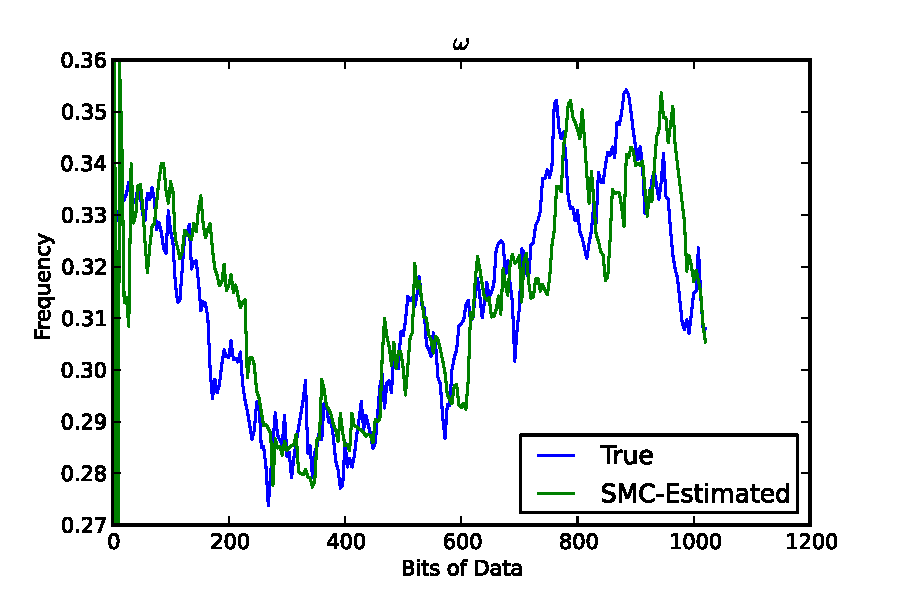
\includegraphics[width=0.6\textwidth]{figures/specdens-tracking}
  \end{figure}

\end{frame}

\begin{frame}{Confidence and Credible Regions}

    Characterizing uncertainty of estimates is critical
    for many applications:

    \only<1>{
      \begin{definition}[Confidence Region]
        $X_\alpha$ is an $\alpha$-confidence region if $\Pr_D(\vec{x}_0 \in X_\alpha(D)) \ge \alpha$.
      \end{definition}
    }

    \only<2->{
      \begin{definition}[Credible Region]
        $X_\alpha$ is an $\alpha$-credible region if $\Pr_{\alert<+->{\vec{x}}}(\vec{x} \in X_\alpha | D) \ge \alpha$.
      \end{definition}
    }

    \uncover<3->{
      Credible regions can be calculated from posterior $\Pr(\vec{x} | D)$
      by demanding
      $$
        \int_{X_\alpha} \dd\Pr(\vec{x} | D) \ge \alpha.
      $$
    }

  \bottomnote{(\emph{Granade} et al. 2012 \shortdoi{s87}; Ferrie 2014 \shortdoi{tb4})}

\end{frame}

\begin{frame}{High Posterior Density}

  Want credible regions that are \emph{small} (most powerful).

  \begin{itemize}
    \item Posterior covariance ellipses (PCE)--- good for approximately normal posteriors
    \item Convex hull--- very general, but verbose description
    \item Minimum volume enclosing ellipses (MVEE)--- good approximation to hull
  \end{itemize}

  \bottomnote{(\emph{Granade} et al. 2012 \shortdoi{s87}; Ferrie 2014 \shortdoi{tb4})}

\end{frame}

\begin{frame}{Comparison of HPD Estimators}

  For multimodal distributions, clustering can be used
  to exclude regions of small support.

  For a noisy coin model (heads probability $p$, visibility $\eta$):

  \begin{figure}
    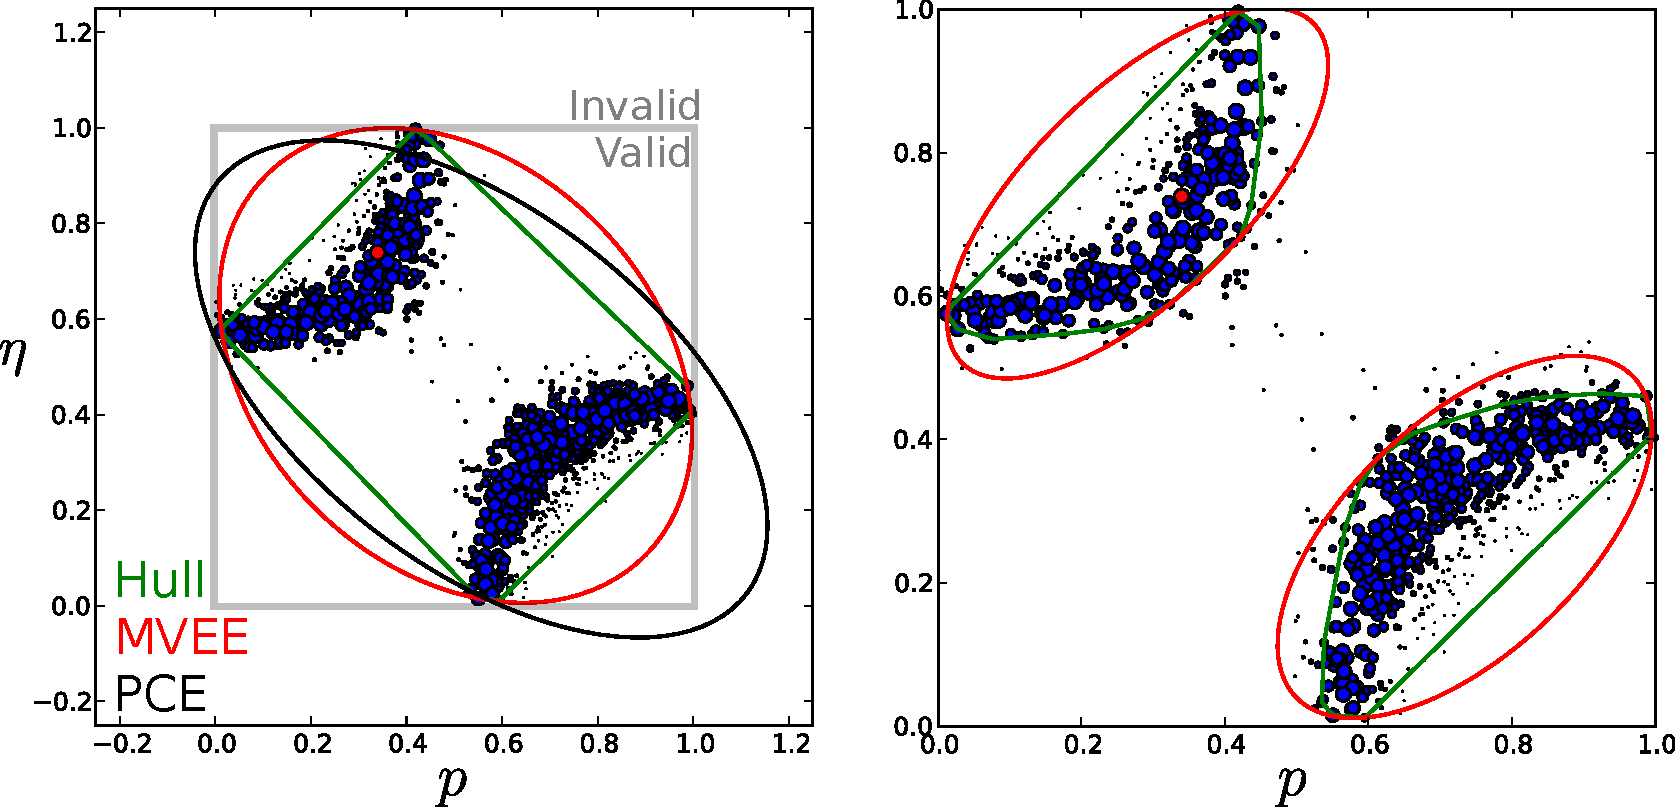
\includegraphics[width=0.6\textwidth]{figures/hpd-clusters}
  \end{figure}

  Left, no clustering. Right, DBSCAN.

  \bottomnote{Plot courtesy of Chris Ferrie. (Ferrie 2014 \shortdoi{tb4})}

\end{frame}

\begin{frame}{Bayes Factors and Model Selection}

  
  \begin{block}{Drunk Under the Streetlights}
    In SMC update $w_i \mapsto w_i \times \Pr(d | \vec{x}; \vec{e}) / \mathcal{N}$,
    $$
      \mathcal{N} = \mathcal{N}(d) \approx \Pr(d | \vec{e}).
    $$
    Is this useful?
  \end{block}

  \pause

  Collecting normalizations $\mathcal{N}_A$ and $\mathcal{N}_B$
  for models $A$, $B$ at each step gives
  $$
    \text{Bayes factor} = \frac{\Pr(D | A; \vec{e}) \Pr(A)}{\Pr(D | B; \vec{e}) \Pr(B)}
    \approx \frac{\prod_{d\in D}\mathcal{N}_A(d)}{\prod_{d\in D}\mathcal{N}_B(d)}
    \times \frac{\Pr(A)}{\Pr(B)} 
  $$

  For full data record, can multiply normalization records to select $A$ versus $B$.

  \bottomnote{(Wiebe, \emph{Granade}, Ferrie and Cory 2014 \shortdoi{tdk})}

\end{frame}

\begin{frame}

  For example, deciding between linear- (left) and complete-graph (right) Ising models:

  \begin{figure}
    \centering
    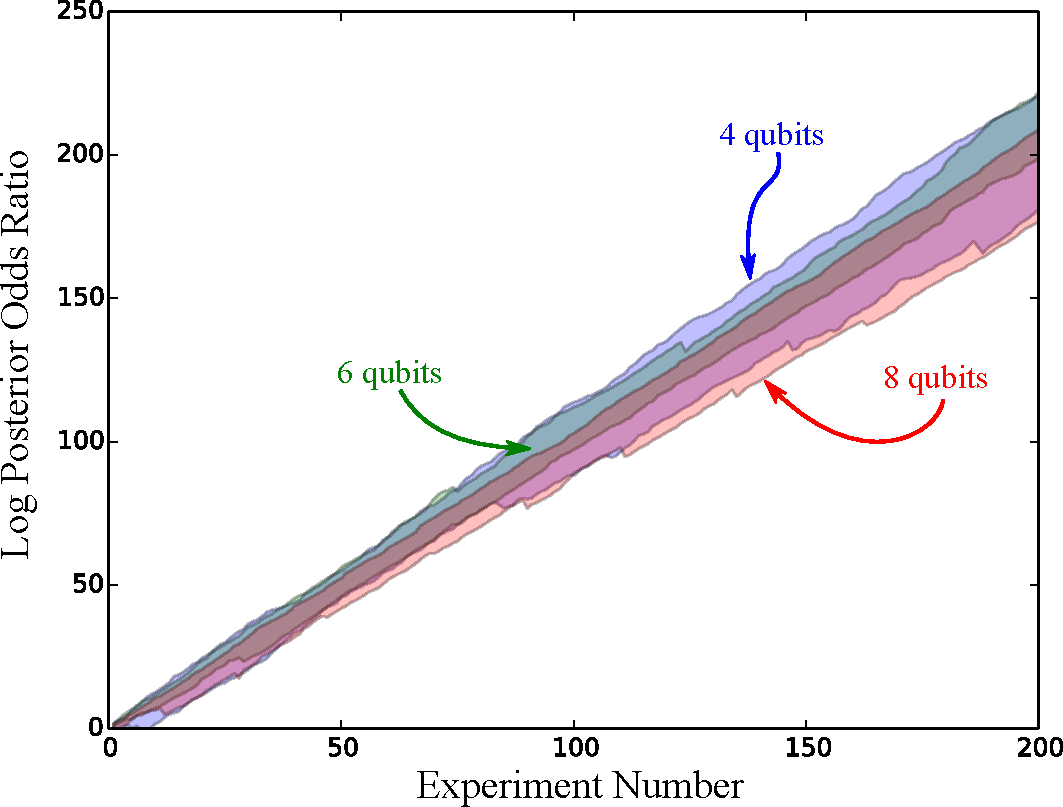
\includegraphics[width=0.425\textwidth]{figures/modelselect_linetrue}
    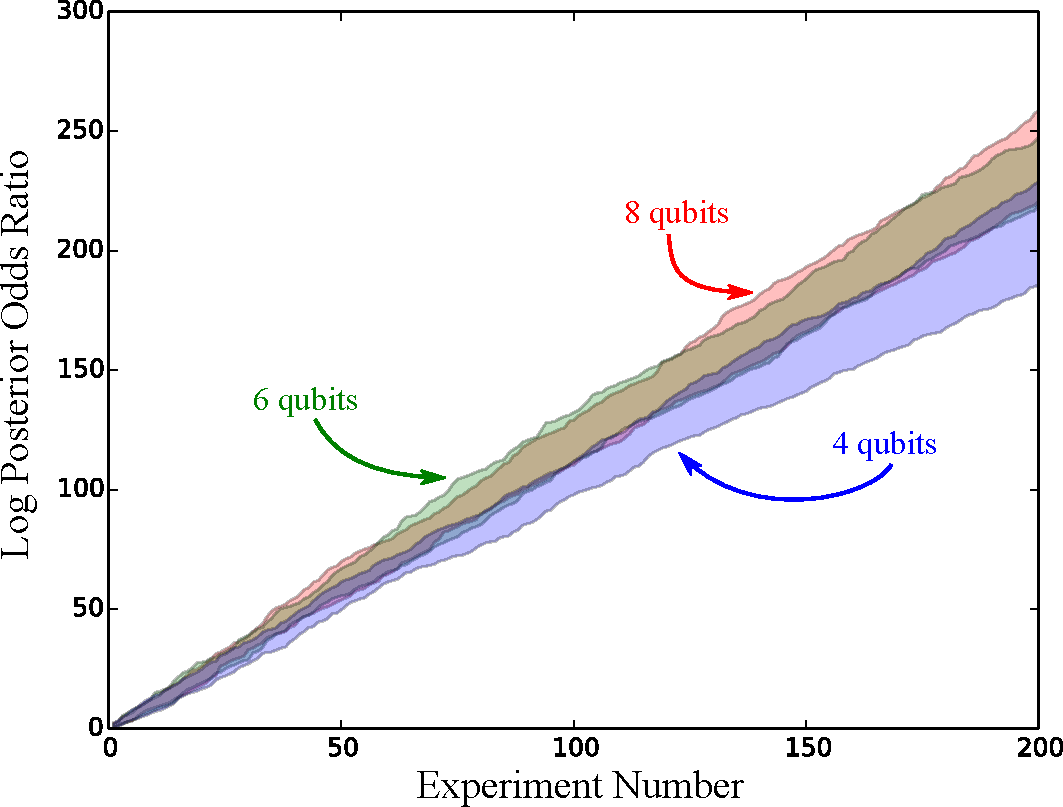
\includegraphics[width=0.425\textwidth]{figures/modelselect_completetrue}
  \end{figure}

  \bottomnote{(Wiebe, \emph{Granade}, Ferrie and Cory 2014 \shortdoi{tdk})}

\end{frame}


\begin{frame}{Method of Hyperparameters}
  
  If ``true'' model $\vec{x} \sim \Pr(\vec{x} | \vec{y})$,
  for some \emph{hyperparameters} $\vec{y}$, can est.
  $\vec{y}$ directly:
  \[
    \Pr(d | \vec{y}; \vec{e}) = \int \Pr(d | \vec{x}, \vec{y}; \vec{e})
      \Pr(\vec{x} | \vec{y}; \vec{e})\ \dd\vec{x}.
  \]

  \pause \vskip0.5em
  
  \begin{example}
    For Larmor precession with $\omega \sim \operatorname{Cauchy}(\omega_0, T_2^{-1})$,
    \[
      \Pr(d | (\omega_0, T_2^{-1}); t) = \ee^{-t T_2^{-1}}\cos^2(\omega_0 t / 2) + (1 - \ee^{-t T_2^{-1}}) / 2.
    \]
    Let $\vec{y} = (\omega_0, T_2^{-1})$.
  \end{example}

  \bottomnote{(\emph{Granade} et al. 2012 \shortdoi{s87})}
  
\end{frame}

\begin{frame}{Hyperparameters and Region Estimation}

  In some hyperparameter models, can also express as region
  estimator on underlying parameters.

  \begin{figure}
    \centering
    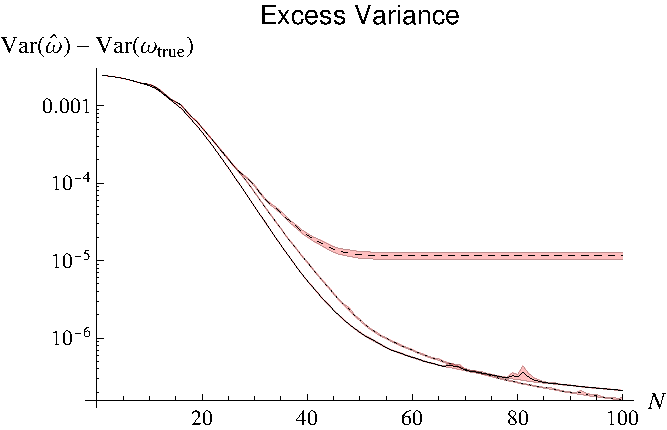
\includegraphics[width=0.5\textwidth]{figures/hypernormal-excess-cov}
    \caption{Larmor precession model w/ $\omega\sim\N(\mu, \sigma^2)$, three exp. design strategies}
  \end{figure}

  Critically, the covariance region for $\omega$ is not smaller
  than the true covariance given by the hyperparameter $\sigma^2$.

  \bottomnote{(\emph{Granade} et al. 2012 \shortdoi{s87})}

\end{frame} 

\end{document}
